\cotefile{93}
\scanpage{92}
% archive foliation: 91
Interprétant $c_{2,3}$ comme
\[
c_{\unsure{2|3},3}:\Omega\unsure{\longrightarrow|\mathbin{-}}\underline{\omega}=\Omega^1_{X/S}
\]
on voit que c'est aussi, compte tenu de
\[
\Omega\simeq\sigma^*(\underline{\Omega}^1_{P/X})
\]
la dérivée relative à la connexion $c$ de la section $\sigma$. on dit (si $\underline{\omega}$ est loc. libre de \unsure{t.f.}) que $\sigma$ (i.e. $\mathcal{L}\subset\mathcal{H}$) est \uline{nulle part stationnaire} pour $c$ si $c_{2,3}$ est ``partout non nulle''. \deleted{\unsure{Appl.}} \inserted{\unsure{i.e.}} $c$ fait de $\Omega$ un facteur direct local de $\underline{\omega}$.

On suppose pour la suite, qu'il en est ainsi, \uline{et} que $\omega$ est inv., \unsure{i.e. encore} que $c_{2,3}:\Omega\longrightarrow\underline{\omega}$ est un iso. On appelle ces connexions ``\uline{transverses} à $\sigma$ (ou à $\mathcal{L}\subset\mathcal{H}$)). On identifie $\Omega\simeq\underline{\omega}$ par $c_{2,3}$, et de façon précise, on suppose donné un iso
\[
\Omega\xrightarrow[\sim]{i}\underline{\omega}=\Omega^1_{X/S}
\]
et on se borne aux conn. pour lesquelles $c_{2,3}=i$. \deleted{\unsure{Elles forment}} \inserted{\unsure{Ce sont les}} sections d'un torseur sous $\mathcal{L}\otimes\underline{\omega}$ [soit $\underline{\operatorname{Conn}}^{\mathrm{trans}}(\mathcal{H},i)$].

Considérons la restriction d'une connexion $c$ à $\Omega\simeq\underline{\omega}=\operatorname{Fil}_1\mathcal{H}$
\[
c|\underset{\substack{\Vert\\\operatorname{Fil}_1\mathcal{H}}}{\Omega}:\quad
\Omega\longrightarrow\underbrace{\mathcal{L}\otimes\omega}_{\unsure{\Omega\otimes\omega,\omega|\Omega^{\otimes2},\omega}}.
\]
\scanpage{93}
% archive foliation: 92
On sait que sa composée avec
\[
\mathcal{L}\otimes\underline{\omega}\longrightarrow\underline{\omega}
\]
est $\unsure{-2i_{\underline{\omega}}|-2\operatorname{id}_{\underline{\omega}}}$. \deleted{\unsure{Considérons}} \unsure{l'hom.} $c|\Omega$.
$c|\underline{\Omega}$ est op. diff d'ordre $\leq1$, on sait qu'il se factorise en
\diagram{\begin{tikzcd}
\underline{\Omega}\arrow[r,"{d^1_{\unsure{\omega}}}","{\substack{\text{op. diff.}\\\text{can.}\\\text{d'ordre }1}}"'] & P^1_{\unsure{X/S}}(\underline{\Omega})\arrow[r,"\gamma","{\uline{\text{lin.}}}"'] & \mathcal{L}\otimes\underline{\omega}
\end{tikzcd}}
et comme la composée
\diagram{\begin{tikzcd}
\underline{\Omega}\arrow[r,"{c|\underline{\omega}}"] & \mathcal{L}\otimes\underline{\omega}\arrow[r] & \underline{\omega}
\end{tikzcd}}
est linéaire (de valeur $-2i$), on trouve que $\gamma$ donne lieu à une hom. d'extensions
\diagram{\begin{tikzcd}
0\arrow[r] & \Omega\otimes\omega\arrow[r]\arrow[d,"{\gamma_0=?}"] & P^1_{X/S}(\Omega)\arrow[r]\arrow[d,"\gamma"] & \Omega\arrow[r]\arrow[d,"{-2i}"] & 0\\
0\arrow[r] & \Omega\otimes\omega\arrow[r] & \mathcal{L}\otimes\omega\arrow[r] & \omega\arrow[r] & 0
\end{tikzcd}}

On va déterminer $\gamma_0$, \unsure{quand on a} splitting $s$ et section $\delta_0$ de $\Omega$, en termes de $\unsure{\omega_0=i|\omega_0=\delta}$, $\omega_1$, $\omega_2$ ci-dessus, \deleted{\unsure{on voit que}} \inserted{En vertu de la} \unsure{recette générale valable pour les op.} $\leq1$ diff.\deleted{\unsure{$P^1_{X/S}(\Omega)\simeq P^1_{X/S}(\mathcal{O}_X)$ et les}}\inserted{sur un $\mathcal{O}_X$-mod. $\Omega$,}
\margin{$\unsure{\delta_0\text{ de }\Omega}$}
ainsi
\[
\gamma(\underset{\in\Omega}{\omega_1}\otimes d\underset{\in\mathcal{O}_X}{f})=c(f\omega_1)-f\,c(\omega_1).
\]
Si $\omega_1=\lambda\delta$, on trouve donc
\[
\begin{aligned}
\gamma(\lambda\delta\otimes df)&=\delta\,[d(f\lambda)-f\,d(\lambda)]\\
&=\delta\,[\lambda\,df]=\lambda\delta\otimes df.
\end{aligned}
\]
donc $\gamma=\operatorname{Id}$. Donc

\uline{Prop.} Si $c$ connexion \uline{transverse}, \inserted{et $2$ inv. sur $X$,} alors $\gamma$ est un \uline{iso} d'extensions de $P^1_{X/S}(\Omega)$
\scanpage{94}
% archive foliation: 93
et $\mathcal{L}\otimes\underline{\omega}$, induisant $-2i$ et $\operatorname{id}$. \unsure{On a} un iso
\[
\mathcal{L}\underset{\gamma^{-1}\otimes\operatorname{id}_{\omega^{-1}}}{\simeq}P^1_{X/S}(\underline{\Omega})\omega^{-1}\simeq P^1_{X/S}(\omega)\omega^{-1}
\]
\deleted{\unsure{Cor.}}
induisant un diagramme d'extensions
\diagram{\begin{tikzcd}
0\arrow[r] & \underline{\omega}\arrow[r]\arrow[d,"\operatorname{id}"] & \mathcal{L}\arrow[r]\arrow[d] & \mathcal{O}_X\arrow[r]\arrow[d,"{-2\operatorname{id}}"{draw,circle}] & 0\\
0\arrow[r] & \underline{\omega}\arrow[r] & P^1_{X/S}(\omega)\omega^{-1}\arrow[r] & \underline{\mathcal{O}}_X\arrow[r] & 0
\end{tikzcd}}
\margin{\textcircled{$\alpha$}}
ou aussi, le multipliant par $-\frac12$
\diagram{\begin{tikzcd}
0\arrow[r] & \underline{\omega}\arrow[r]\arrow[d,"{-\frac12\operatorname{id}_{\omega}}"{draw,circle}] & \mathcal{L}\arrow[r]\arrow[d] & \mathcal{O}_X\arrow[r]\arrow[d,"{\operatorname{id}_{\mathcal{O}_X}}"] & 0\\
0\arrow[r] & \underline{\omega}\arrow[r] & P^1_{X/S}(\omega)\omega^{-1}\arrow[r] & \mathcal{O}_X\arrow[r] & 0
\end{tikzcd}}
\margin{\textcircled{$\unsure{\alpha'|\beta}$}}

(Donc le torseur sous $\underline{\omega}\simeq\Omega$ \unsure{définissant} l'ext. $\mathcal{L}$ est déduit du torseur \inserted{\unsure{sous $\omega$}} défini \inserted{par l'ext.} $(P^1_{X/S}(\underline{\omega})\underline{\omega}^{-1}$ de $\mathcal{O}_X$ par $\underline{\omega}$ (ou $P^1_{X/S}(\omega)$ de $\underline{\omega}$ par $\underline{\omega}^2)$ \uline{par multiplication par $-2$}.

Utilisant ces hom. comme identifications,
$c|\underset{\substack{\Vert\\\operatorname{Fil}_1\mathcal{H}\\\Vert\\\mathcal{L}^{\unsure{\mathrm{ab}}}}}{\underline{\Omega}\simeq\underline{\omega}}$ s'identifie à l'op. diff. universel,
\[
d^1_{\underline{\omega},X/S}\quad
\underset{\substack{\Vert\\\omega}}{\Omega}\xrightarrow{c}\mathcal{L}\otimes\omega\simeq P^1(\omega)
\]

\uline{NB} On utilisera \unsure{l'iso} comme identification et on se borne aux conn. de $\mathcal{H}$, donc $c:\mathcal{H}\longrightarrow\mathcal{H}\otimes\omega$, dont la restriction à $\underline{\Omega}\simeq\underline{\omega}=\unsure{\mathcal{L}_{\omega}}$ est le $d^1_{\underline{\omega},X/S}$.
\deleted{Ils sont déterminés \unsure{par une}} \deleted{\unsure{famille}} \inserted{\unsure{section}} \unsure{donnée à} $\underline{\Omega}\otimes\omega\simeq\underline{\omega}^{\otimes2}$.
\scanpage{95}
% archive foliation: 94
Donc pour la suite on se donne d'abord l'extension
\[
0\longrightarrow\Omega\longrightarrow\mathcal{L}\longrightarrow\underline{\mathcal{O}}_X\longrightarrow0
\]
\margin{On suppose $2$ inv. sur $X$}
($\Omega$ inversible), puis l'op. diff. d'ordre $\leq1$
\[
\Omega\xrightarrow{c_\Omega}\mathcal{L}\otimes\underline{\omega}\qquad\underline{\omega}=\Omega^1_{X/S}
\]
tel que

a) le composé avec $\mathcal{L}\otimes\underline{\omega}\longrightarrow\underline{\omega}$ soit \deleted{\unsure{un}} $\Omega\longrightarrow\underline{\omega}$ linéaire et un \uline{iso} (qu'on notera $-2i$, $i:\Omega\simeq\underline{\omega}$ qu'on utilisera parfois pour identifier)
\margin{\unsure{cela a l'air vraiment vicieux vrai}}

b) \deleted{\unsure{L'hom.}} On a (si $w\in\Gamma\Omega$, $f\in\Gamma\underline{\mathcal{O}}_X$)
\[
c_\Omega(fw)-f\,c_\Omega(w)=w\otimes df
\]
($w$ fixé, \unsure{c'est bien} \uline{lin.} $\Omega\longrightarrow\Omega\otimes\omega$)

[Ces conditions définissent le \unsure{système} de l'ext. $\mathcal{L}$ et de l'op. diff $c_\Omega$ à isom unique près -- et on peut tjrs en trouver, si $\underline{\omega}=\Omega^1_{X/S}$ est bien inversible)

On forme $\mathcal{H}$, et on considère les connexions \inserted{\unsure{\(\mathcal{H}\)}} d'alg. de Lie \deleted{\unsure{\(\mathcal{H}\)}} sur $\mathcal{H}$ qui prolongent $c_\Omega$. Elles forment les sections d'un torseur sous $\unsure{\Omega^2}\otimes\underline{\omega}\simeq\underline{\omega}^{\otimes\unsure{2|3}}$. \deleted{On se demande quelles}

\margin{La donnée de $c_\Omega$ revient à celle d'un iso. des voisinages infinitésimaux d'ordre $2$ de $\sigma(X)$ dans $P$ et de $\Delta_X(X)$ dans $X\times_S X$. $\unsure{\longrightarrow}$ celle de $c_{\mathcal{H}}$ les \deleted{\unsure{prolongeant à un iso des}} voisinages d'ordre $3$ les prolongeant (et alors, un iso des \unsure{vois. form.})}

Faire le lien avec la situation $(P,\sigma,c)$ et les données formelles
\[
\underline{\mathcal{O}}_{\widehat P}^{\mathrm{con}}\simeq P^\infty_{X/S}
\]
(si $X/S$ de \unsure{f.t.} lisse --).
\scanpage{96}
% archive foliation: 95
\uline{1.5.}\quad\uline{Sections horizontales de} $P$

Pour quelles connexions projectives sur $X/S$ (avec $\underline{\omega}_{X/S}$ inv.) y a-t-il des sections horizontales \inserted{de $P$,} et quelles sont-elles ? On va étudier d'abord les sections horizontales de $P$ là où elles sont disjointes de la section donnée $\sigma$. Elles correspondent donc à une décomp. de $\mathcal{L}$ en somme directe, ou de $\mathcal{H}$ en
\[
\mathcal{H}\simeq\Omega\oplus\Omega^0\oplus\Omega^{-1}\qquad(\Omega\simeq\omega)
\]
\deleted{Si la \unsure{connexion}} Une connexion $c$ \unsure{donne} la section $\sigma'$ horizontale \unsure{ssi} \deleted{$c(\Omega^{-1})\subset$}
\[
c(\Omega^{-1})\subset(\Omega^0+\Omega^{-1})\otimes\underline{\omega}
\]
\inserted{ou $c(\Omega^0)\subset(\Omega^0+\Omega^{-1})\otimes\underline{\omega}$}
\margin{$\uline{2\text{ inv.!}}$}
\unsure{comme la donnée} d'une \deleted{section}\inserted{base} $\delta$ de $\Omega$, permettra de décrire $c$ par trois formes $\bar\omega_2$, $\bar\omega_1$, $\bar\omega_0$, à valeurs dans $\Omega\otimes\underline{\omega}$, $\Omega^0\otimes\underline{\omega}=\underline{\omega}$ et $\Omega^{-1}\otimes\underline{\omega}$ :
\[
-\unsure{2}\bar\omega_2=0
\]
\deleted{donc si $2$ inversible ceci signifie $\bar\omega_2=0$} et peut donc s'obtenir (si un \unsure{choix} de connexion \unsure{mod} $\Gamma(\Omega\otimes\omega)$ est donné) \deleted{\unsure{précis.}} \inserted{\unsure{préc.}} \unsure{par la} restriction à $\Omega$ -- puis on obtient de façon unique en corrigeant $c$ par adjonction d'une $\omega_2\in\Gamma\Omega\otimes\underline{\omega}$.

Donc

\uline{Prop.} Pour tout splitting de \inserted{l'ext.} $\mathcal{L}$ ($\simeq P^1_{X/S}\underline{\omega}\otimes\underline{\omega}^{-1}$ dans le cas ``canonique'') il y a une et une seule \uline{conn. admissible} sur $\mathcal{H}$ (ou $P$ --) pour laquelle la section correspondante de $P$ soit horizontale. Donc \deleted{\unsure{caractérisation bien}} \deleted{une} \deleted{injection}\inserted{application} de l'ens. des sections de $P-\sigma(X)$ sur $X$, \inserted{i.e. des splittings de $P^1_{X/S}(\omega)$,} dans l'ens. des connexions \deleted{\unsure{différentielles}} sur $X$, ayant comme image celles qui admettent une section hor. disjointe de $\sigma$.
\scanpage{97}
% archive foliation: 96
Quelles connexions \unsure{affines} obtient-on ainsi ?
\deleted{Choisissons (localt) une \unsure{uniformisante} $t$ de $X$, d'où une base $dt$ de $\omega\simeq\Omega$, et un splitting de $P^1_{X/S}(\Omega)\simeq P^1_{X/S}(\omega)\simeq P^1_{X/S}(\mathcal{O}_X)$ (par le choix de la base $dt$), d'où une connexion \inserted{projective} correspondante.}
On peut supposer $\mathcal{H}$ splitté localement, avec base $\delta$ de $\Omega$, et une connexion de référence $c_0$ décrite par
\[
\begin{aligned}
c_0(\underset{\substack{\Vert\\\lambda\delta}}{\omega_1})&=\delta\,d\lambda+\omega_1(-2\bar\omega_0),&\bar\omega_0&\in\Gamma\Omega^{-1}\otimes\omega^{\unsure{1}},\\
c_0(\underset{\substack{\Vert\\\mu\cdot1}}{\omega_0})&=1\,d\mu+\omega_0(\bar\omega_0),\\
c_0(\underset{\substack{\Vert\\\unsure{\gamma|\nu}\delta^{-1}}}{\omega_{-1}})&=\delta^{-1}d\unsure{\gamma|\nu}\,\deleted{\unsure{\omega}}.
\end{aligned}
\]
Considérons une section $s$ de $\mathcal{L}$ s'envoyant sur section $1_X$ de $\mathcal{O}_X$
\[
s=s_0+\omega_1\qquad(s_0=(0,1))
\]
soit
\[
\left\{\begin{array}{l}
\deleted{\unsure{\psi_s}:\mathcal{O}_X\longrightarrow\mathcal{L}}\\
\nu_s:\Omega^{-1}\longrightarrow\mathcal{H}
\end{array}\right.
\qquad\text{i.e. }\nu_s\in\Gamma(\mathcal{H}\otimes\Omega)
\]
\margin{\deleted{\unsure{$\psi_s\in\Gamma(\mathcal{L})$}}}
\deleted{l'élément}\inserted{l'hom} correspondant. \deleted{\unsure{et}} On a
\[
\deleted{s=\exp\Theta_{\omega_1}\cdot s_0=s_0+[-\omega_1,s_0]+\unsure{[-\omega_1]}}
\]
\[
\nu_s=\exp\Theta_{\omega_1}\nu_{s_0}
=\nu_{s_0}+\underbrace{[-\omega_1,\nu_{s_0}]}_{\unsure{-2\omega_1\nu_{s_0}}}
+\underbrace{\frac12[-\omega_1,[-\omega_1,\nu_{s_0}]]}_{\unsure{+\omega_1^2\nu_{s_0}}}
\]
\margin{\unsure{pour $s_0=s$}}
\deleted{d'où la question est si $c(\nu_s)$ est} de calculer la composante \inserted{$\bar\omega_2(s)=\varphi(\omega_1)$} de $c(s)$, suivant la \deleted{base}\inserted{$\Omega\otimes\omega$} \deleted{\unsure{que la}} décomposition
\[
\mathcal{H}\simeq\Omega+\deleted{\unsure{\exp\Theta}}\mathcal{O}_X\cdot s+\nu_s(\Omega^{-1})
\]
i.e.
\[
(\exp\Theta_{\omega_1})\otimes\operatorname{id}_{\omega}\bigl(c(s)\bigr).
\]
\deleted{et la forme cherchée (pour corriger) est}
\[
\deleted{\unsure{\bar\omega_2(s)=-\varphi(\omega_1)\in\Omega\otimes\omega}.}
\]
\[
\deleted{\underbrace{c(\nu_s)=\bar\omega_2(s)+\unsure{\bar\omega_1(s)}\,\unsure{s\otimes\bar\omega_1(1)}+(\nu_s\otimes\operatorname{id})(\bar\omega_{-1})}_{\substack{\Omega\otimes\omega\qquad\omega\qquad\Omega^{-1}\otimes\omega\\=\text{composante de }\exp\Theta_{+\omega_1}(c(s))}}}
\]
\margin{\deleted{$\unsure{\operatorname{id}\otimes c(s_0)}$}\inserted{$\unsure{-\omega_1}$}}
Sauf erreur, on trouve
\[
s=s_0+\omega_1\longmapsto c_0+\bigl(\delta\,d(\unsure{\omega_1\delta^{-1}})+\omega_1^2\bigr).
\]

% right half, continuing the left half
Prenons $\delta$ de façon que son image dans $\omega$ soit $dt$, $t$ une uniformisante, on trouve sauf erreur de calcul --
\[
s_0+\lambda\,dt\longmapsto c_0^{\deleted{\unsure{dt}}}+\left(\frac{d\lambda}{dt}+\lambda^2\right)(dt)^2
\]
\margin{facteur $2$ !}
Donc quand une conn. proj. sur $X/S$ est définie par (\unsure{au-delà} de la \deleted{forme}\inserted{conn.} proj. de réf. $c_0$) par une $2$-forme $\varphi(dt)^2$, la question si on peut trouver une section horizontale de $P$ disjointe de la section donnée revient à celle de trouver des solutions $\lambda$ de l'équation
\[
\frac{d\lambda}{dt}+\lambda^2=\varphi
\]
(équation diff. non lin. du $1^{\mathrm{er}}$ ordre). On sait, si $X$ courbe lisse sur corps $k$ de car nulle, qu'il y a au plus une solution ayant une valeur et une dérivée données en un pt; \unsure{s'il y en a une infinité}, mais transcendantes (!), en \uline{algébrique} on peut \unsure{avoir} --

Les pôles de $\lambda$ \inserted{\unsure{nous}} correspondent à des pts de rencontre de $\sigma$ \inserted{section} (défini par $\lambda$) et de $\sigma'$ --

\uline{1.6.} Intrinsèquement, le $P$ canonique est $\simeq\mathbb{P}(P^1_{X/S}(\underline{\omega}))$, où $\underline{\omega}=\underline{\Omega}^1_{X/S}$. Donc une section de $P$ s'identifie à un couple
\[
(L,\gamma)
\]
$L$ Module inversible sur $X$, et
\[
\gamma:P^1_{X/S}(\omega)\longrightarrow L\qquad\text{épi. lin.}
\]
Or un hom. \deleted{\unsure{lin.}}\inserted{\unsure{l'op.}} $\gamma:P^1_{X/S}(\omega)\longrightarrow L$ équivaut à
\scanpage{98}
% archive foliation: 97
un op. \unsure{1-diff.} (rel. à $X/S$)
\[
D:\underline{\omega}\longrightarrow L,
\]
\deleted{satisfaisant}
et la restriction de $\gamma$ à $\underline{\omega}\otimes\underline{\omega}=\underline{\omega}^2\subset(P^1_{X/S}\omega)$
\[
\gamma_0:\underline{\omega}^2\unsure{\text{---}|\longrightarrow}L\qquad\text{i.e. }\gamma_0\in\Gamma(L\otimes\omega^{-2})
\]
est aussi définie par
\[
D(f\omega)-fD(\omega)=\gamma_0(\omega\cdot df)
\]
($\omega\in\Gamma\underline{\omega}$, $f\in\Gamma\underline{\mathcal{O}}_X$). Les pts où la section $\sigma'$ déduite de $\gamma$ (ou $D$) rencontre la section $\sigma$ canonique sont ceux où $\gamma_0$ s'annule, i.e. les \uline{pts de dégénérescence} de l'op. diff. $D$. On notera qu'aux pts de non dég., il est automatique que $\gamma$ est épi -- que ce soit épi en tt pt signifie aussi que $L$ est engendré comme module par les $D(\omega)$ ($\omega$ sections locales de $\underline{\omega}$). Si ce n'est pas vrai, alors (si $X$ courbe alg. sur corps de base $k$) il y a un sous-Module $L'\subset L$ canonique par lequel se factorise $D$ (le plus petit --) qui est inv. et pour lequel la condition est vérifiée --

On voit donc qu'à tt tel épi est associée, \uline{sur l'ouvert des pts où elle est non dégénérée}, une connexion projective \deleted{\unsure{qui}} unique qui la rende horizontale. \deleted{La question si $\exists$ connexion}
\scanpage{99}
% archive foliation: 98
Pour que la section donnée $\sigma'$ de $P$ soit horizontale pour une conn. proj. $c$ convenable il f. et s. \unsure{a)} que l'ouvert $U$ des pts où $D$ est non dég. soit dense sur chaque fibre de $X$ sur $S$ et b) que la section qu'on vient de définir \inserted{sur $U$} du Torseur $\uline{\operatorname{Connproj}}$ sous $\underline{\omega}^2$ \deleted{\unsure{sur}} ``soit régulière sur tt $X$'' (i.e. se prolonge \inserted{en section régulière} sur tt $X$ laquelle sera unique). Cette condition est une condition purement locale en les pts de \deleted{\unsure{pôles}} \deleted{\unsure{dégénérescence, et signifie}} dégénérescence, et signifie qu'en termes d'un \unsure{splitting} de $P^1_{X/S}\underline{\omega}$, $\gamma$ \deleted{\unsure{il}} doit avoir une singularité polaire au plus d'ordre $1$, et la partie \deleted{polaire} \deleted{\unsure{et la}} principale polaire à l'ordre $1$ près comme section nulle au pt envisagé doit être déterminée ! (écrire que $\lambda^2+\frac{d\lambda}{dt}$ n'a pas de pôle en un pt où $\lambda$ \deleted{\unsure{peut en avoir}}\inserted{en a} un !).

Donc, le long de la section marquée $\sigma$ de $P$, il y a un champ d'éléments de section d'ordre $2$ transverses à $\sigma$, et les sections $\sigma'$ de $P$ \inserted{sur $X$} pour lesquelles il y a une connexion projective de $X$ rendant $\sigma'$ horizontale (laquelle sera unique) sont celles qui, aux pts d'intersection avec $\sigma$, ont \deleted{\unsure{un}}\inserted{comme} jet d'ordre $2$ celui du champ. [\uline{NB} des élts de contact can. d'ordre $1$ à trouver \unsure{chaque} fois qu'on prend un $\Omega$ inversible, et la section de $\mathbb{P}(P^1_{X/S}(\Omega))$ définie par la
\scanpage{100}
% archive foliation: 99
structure d'extension de $P^1_{X/S}(\Omega)$, --- plus gén., chaque fois qu'on a une ext. de $\Omega$ inv. par $\Omega\otimes\omega$, $\underline{\omega}=\Omega^1_{X/S}$ inversible aussi\ldots

Si l'op. diff. $\omega\longrightarrow\underbrace{L\simeq\underline{O}_X}_{\unsure{\text{par choix loc.t}|\text{pour choix local}}}$ est
\[
D(f\,dt)=a\frac{df}{dt}+b
\]
la \unsure{coordonnée principale} est $\dfrac ba=\lambda_t$
(on dépend ici du choix de l'uniformisante $t$)
et la condition, en un pôle de $\lambda$ i.e. zéro de $a$
(qui donc ne doit pas être zéro de $b$, car $a$ et $b$ ne doivent pas être nuls simultanément) est

\noindent a) $\lambda_t$ \deleted{est} n'a que pôles simples

\noindent b) \deleted{$\unsure{\beta}$} $\lambda_t$ a comme développement formel en $t$
\[
\lambda_t=\frac{2}{t}\;(+\text{ pas de terme constant})+\text{termes d'ordre }\uline{\geq1}.
\]
\scanpage{101}
\mspage{1}
% archive foliation: 100
\deleted{\diagram{\begin{tikzcd}
\mathcal M_g^{\unsure{G|4}}\arrow[r]&\mathcal M_g&\mathcal M_{g\unsure{c}}\arrow[ll,bend left=40,swap,"{\unsure{\text{ret. à }}\uline{\unsure{\text{H}^{1}\text{ sur fibres}|\text{H sur fibres}}}}"]\quad(\text{avec conn. aff.})
\end{tikzcd}}}
\[
P=\mathbf P(P^1_{X/S}(\underline\omega)),\ \sigma,\ c
\qquad\unsure{\text{---}|\longrightarrow}\quad\sigma,\ c+\bar\omega_2,\quad\bar\omega_2\ne0
\]
\unsure{Autom.} de $P$ transforme $c$ en $c+\bar\omega_2$

\unsure{car} \uline{\unsure{Uniquement}} $\unsure{1\ne}$ \unsure{autom.}
Quels sont les autom. $\unsure{u}$ de $P$ tels que $u(c)$ soit de la forme $c+\bar\omega_2$ ??

\margin{$\unsure{\omega}$}
\margin{$\unsure{-}\omega\subset\mathcal L\subset\mathcal H\ \unsure{a}$}

\uline{Sections de $P$} disjointes de $\sigma$ = splitting de $\mathcal L$
\[
=\text{splitting de }P^1_{X/S}(\underline\omega)
=\text{connexion sur }\omega
\]
\deleted{\unsure{forme un torseur de $\omega$}}
\uline{ou} op. diff. d'ordre 1 sur $\omega$ à valeurs dans $\omega\otimes\omega=\omega^2$

\deleted{\uline{Connexions projectives}, \unsure{s'interprètent comme}}
\deleted{\unsure{sections}}
\[
D(f\omega)-fD(\omega)=\omega\otimes df
\]
\[
D\,f\,dt=f\underbrace{D(dt)}_{\lambda}+dt\,df
\]
Sections de $P$ non disjointes de $\sigma$ = connexions de $\omega$ avec \deleted{\unsure{points}} \uline{singularités} polaires

Connexions projectives de $P$ = \deleted{conditions} différentielles du premier ordre sur sections de $P$ i.e. sur connexions de $\omega$, de la forme\ldots ?
\[
0\longrightarrow\underbrace{\omega\subset\mathcal L}_{O}\subset\mathcal H\longrightarrow0
\]
\[
s:\underline\omega^{-1}\longrightarrow\mathcal H
\qquad
\nu_s\in\Gamma\,\mathcal H\otimes\underline\omega
=\underline\omega^{\unsure{2|1}}\oplus\underline\omega\oplus\underline\omega^0
\qquad\unsure{\nu_s}=0+0+1
\]
\[
\underline\omega+\underline O_X\cdot s+\nu_s(\underline\omega^{-1})
\qquad c(s)\subset\unsure{\Omega|\mathcal L}\otimes\omega+\nu_s\cdot\underline O_X\ ?
\]
\[
\omega_{\unsure{a}}+\underline O_s+\omega'
\qquad \deleted{\unsure{\lambda}}\quad
c(s)=\bar\varphi_2+s\otimes\bar\varphi_1+\nu_s\cdot\bar\varphi_0
\quad\underbrace{\text{avec }\unsure{\bar\omega_0}=0\ ?}
\]
\[
s=s_0+a_1\quad(a_1\in\Gamma\underline\omega)
\]
\[
\begin{aligned}
\bigl(\exp(\Theta_{a_1})\otimes\mathrm{id}_{\underline\omega}\bigr)^{\unsure{-1}}c(s)
&=\bar\varphi_2+(\exp(\Theta_{a_1})s)\otimes\bar\varphi_1
 +(\exp\Theta_{a_1}\,\unsure{\omega|\nu_s})\unsure{\bar\varphi_0}\\
&=\bar\varphi_2+s_0\bar\varphi_1+\bar\varphi_0
\end{aligned}
\]
\scanpage{102}
\mspage{5}
% archive foliation: 101
\[
\frac{dt}{ds}=\frac1{ds/dt}=\frac1{s'}\qquad ds=s'\,dt
\]
\[
\deleted{\unsure{dt/ds}}\qquad d\frac{dt}{ds}=-\frac{s''}{s'^2}\,dt
\qquad ds\,d\frac{dt}{ds}=-\frac{s''}{s'}\,dt^2
\]
\[
c_{D_s}=c_{D_t}-2\left(\frac{s''}{s'}\right)'dt^2+\left(\frac{s''}{s'}\right)^2dt^2
\]
\[
\boxed{c_{D_s}=c_{D_t}+\left[-2\left(\frac{s''}{s'}\right)'+\left(\frac{s''}{s'}\right)^2\right]dt^2}
\]
\[
\left[\text{où }s'=\frac{ds}{dt},\ s''=\frac{ds'}{dt},\quad
\left(\frac{s''}{s'}\right)'=\frac d{dt}\left(\frac{s''}{s'}\right)\right]
\]
\[
[\quad]=-2\frac{s'''s'-s''^2}{s'^2}+\frac{s''^2}{s'^2}
=\frac{3s''^2-2s's'''}{s'^2}
\]
\[
\boxed{c_{D_s}=c_{D_{\unsure{t|\sigma}}}+\frac{3s''^2-2s's'''}{s'^2}dt^2}
\]
\unsure{On doit|On cherche} $c_{D_s}=c_{D_t}$ ssi \uline{ou bien} $s''\equiv0$ i.e. $s$ lin. en $t$, ou bien
\[
3s''^2=2s's'''\quad\text{i.e. }\unsure{2}\frac{s'''}{s''}=\frac32\frac{s''}{s'}
\]
\[
\text{i.e. }(\log s'')'=\left(\frac32\log s'\right)'
\]
\[
\text{i.e. (car. 0) }2\log s''=\unsure{\frac32|3}\log s'+\underbrace{c^{te}}_{\deleted{\unsure{\mathrm{cte}}}}
\]
\[
\log\frac{s''^2}{s'^3}=c^{te}
\]
\margin{$s$ \unsure{fct homographique} de $t$ !}
\[
\frac{s''^2}{s'^3}=c^{te}\quad\text{i.e.}\quad s''^2=C^{\unsure{te}}s'^3
\qquad s''=C\,s'^{3/2}
\]
\[
s=\frac{at+b}{ct+d}=\deleted{\unsure{u_t}}\,u_M(t)\qquad
M\text{ la matrice }\begin{pmatrix}a&b\\c&d\end{pmatrix}
\]
\[
D_{u_M(t)}=D_t
\]
On peut se réduire aux 3 types \unsure{d'hom.}
\[
\begin{gathered}
t\longmapsto t+a\\
t\longmapsto bt\\
t\longmapsto\frac1t
\end{gathered}
\]
\[
s=\frac1t,\quad s'=-\frac1{t^2},\quad s''=+\frac2{t^3},\quad s'''=-\frac6{t^4}
\]
\[
3s''^2-2s's'''=\frac{12}{t^6}-\frac{12}{t^6}=0
\]
\scanpage{103}
\mspage{2}
% archive foliation: 102
\[
\underline\omega+\underline O_Xs_0+\underline\omega^{-1}\nu_{s_0}
\]
\[
s=s_0+a_1=(\exp\Theta_{-a_1})s_0=s_0+[-a_1,s_0].
\]
\[
\left[\begin{aligned}
\nu_s&=(\exp\Theta_{-a_1}\otimes\mathrm{id}_{\underline\omega})\nu_{s_0}
=1+\underbrace{[-a_1,\nu_{s_0}]}_{-2a_1\unsure{\nu_{s_0}}}
+\frac12\underbrace{[-a_1,\underbrace{[-a_1,\nu_{s_0}]}_{-2a_1}]}_{-\unsure{2}a_1^2}\\
\nu_s&=\deleted{\unsure{a}}\underbrace{-a_1^2}_{2}\underbrace{-2a_1}_{1}+\underbrace{1}_{0}
\end{aligned}\right]
\]
Il faut calculer, pour avoir l'équation d'horizontalité sur $s$ (ou sur $a_1$) relative à $c$, la \deleted{\unsure{coefficient}}\inserted{composante} dans $\underline\omega^2$ (première comp.) de
\[
(\exp(\Theta_{a_1})\otimes\mathrm{id}_{\underline\omega})(c(s))
\]
et l'égaler à 0.

\deleted{On \unsure{supp. $c$ provenant d'une conn. $c$ associée} à un splitting, i.e. pour lequel ce splitting est horizontal}
\deleted{$c(s)=c(s_0)+c(a_1)$}
\[
c(s_0)=\deleted{\unsure{\bar\varphi_1+\nu_{s_0}}}\bar\varphi_2+\nu_{s_0}
\]
\[
(\exp\Theta_{a_1}\otimes\mathrm{id}_{\underline\omega})
\underbrace{(c(s))}_{\substack{c(s_0)+c(a_1)\\=\bar\omega_2+c(a_1)+\nu_{s_0}}}
\quad\deleted{\unsure{+}}(\exp\Theta_{a_1}\otimes\mathrm{id}_{\underline\omega})(\unsure{a_1})+{}
\]
\unsure{est sa comp.} dans $\underline\omega^2$, et si
\[
c(a_1)=\deleted{\unsure{\omega}}\underbrace{\overbrace{D_1(a_1)}^{2}}_{\substack{\text{op. diff. d'ordre}\\1\quad\underline\omega\longrightarrow\underline\omega^2}}
-\overbrace{2a_1}^{1}+\deleted{\unsure{\nu_{s_0}}}\ (\deleted{\unsure{\exp\Theta\omega}}\ldots
\]
\margin{pour un splitting convenable \inserted{et une base $\delta$ de $\omega$}, \deleted{\unsure{si on a}} on a $D_1(\delta)=0$ i.e. $D_1(\lambda\delta)=\delta\,d\lambda$}
On a donc
\[
\begin{aligned}
(\exp(\Theta_{a_1})\otimes\mathrm{id}_{\underline\omega})(c(s))
&=\inserted{\underline\omega_2+{}}\overbrace{D_1(a_1)}^{2}-\overbrace{2a_1}^{1}
-\underbrace{\overbrace{2[a_1,a_1]}^{2}}_{+2a_1a_1}\\
&\qquad\deleted{+2\unsure{a}}\underbrace{-a_1^2}_{2}+2a_1+1
\end{aligned}
\]
L'équation est donc
\[
\boxed{D_1(a_1)+a_1^2\unsure{-|+}\underline\omega_2=0}
\]
\margin{\unsure{facteur 2 qui manque avant ce calcul ?}}
\margin{équation d'horizontalité de la section de $P$ \unsure{disjointe} de $\sigma$, définie par la 1-forme $a_1$}
Si on choisit convenablement une base de $\omega$ (p. ex. $\delta=dt$) on peut supposer $D_1(\delta)=0$ et l'équation en termes de $a_1=\lambda\delta$ est
\[
(d\lambda)\delta+\lambda^2\delta^2=0
\]
ou encore, si $\delta=dt$ i.e. $a_1=\lambda\,dt$
\deleted{$\unsure{\frac{d\lambda}{dt}+\lambda}$}
\[
\boxed{\frac{d\lambda}{dt}+\lambda^2=A}
\]
\margin{TSVP}
\scanpage{104}
\mspage{2 bis}
% archive foliation: 103
Quand on change de connexion projective cela revient simplement \deleted{\unsure{devoir}}\inserted{à} changer le second \unsure{mb.} de l'équation.
\scanpage{105}
\mspage{3}
% archive foliation: 104
Sections de $P-\sigma(X)$ = connexions sur $\omega$
\[
=\text{op. [diff. d'ordre 1] }\underline\omega\longrightarrow\underline\omega^{\unsure{2}}\deleted{\unsure{\omega}}
\]
satisfaisant $D(f\omega)=fD\omega+\omega\,df$
\unsure{forme} torseur sous $\underline\omega$

À toute telle section correspond une connexion projective particulière $c_D$ --- l'unique conn. projective pour laquelle cette section est horizontale.
Si on se fixe une section du \inserted{$P-\sigma(X)$, i.e. une section du} torseur des connexions sur $\underline\omega$ \inserted{\unsure{i.e. si on a une connexion} $D_1:\omega\longrightarrow\omega^2$}, i.e. un splitting de $\mathcal L$ (ou encore de $\mathcal H$\ldots), soit $D_0$\deleted{\unsure{D}}, \deleted{ce qui donne lieu à \unsure{une appl. de}}
\[
\boxed{c_{D_0+\underbrace{\underline\omega_1}_{\text{entrée}}}=\deleted{\unsure{D_0(\omega_1)+\omega_1^2}}c_{D_0}+2D_0(\omega_1)+\omega_1^2}
\]
\unsure{Et vérifions}
\[
\begin{aligned}
c_{D_0+\omega_1+\bar\omega_1}
&=\underbrace{c_{D_0+\omega_1}}_{c_{D_0}+\unsure{D_0\omega_1}+\omega_1^2}
+\underbrace{(D_0+\omega_1)(\bar\omega_1)+\bar\omega_1^{\unsure{2|1}}}_{2D_0(\bar\omega_1)+2\omega_1\bar\omega_1+\bar\omega_1^2}\\
&=c_{D_0}+2D_0(\omega_1+\bar\omega_1)+\omega_1^2+\bar\omega_1^2+2\omega_1\bar\omega_1\\
&=c_{D_0}+2D_0(\omega_1\unsure{+|,}\bar\omega_1)+(\omega_1+\bar\omega_1)^2\qquad\text{OK}
\end{aligned}
\]
Équation d'horizontalité de $D_0+\omega_1$ pour une connexion proj. $c_{D_0}+\bar\omega_2$ :
\[
c_{D_0}+\bar\omega_2=c_{D_0+\omega_1}\quad\text{i.e.}
\]
\[
\boxed{2D_0(\omega_1)+\omega_1^2=\bar\omega_2}
\]
\unsure{Considérons} la connexion
\[
D_t(\lambda\,dt)\longrightarrow\frac{d\lambda}{dt}dt^2\quad\text{i.e.}
\]
Ou :
\[
D_t(\omega)=\left(\frac d{dt}\left(\frac\omega{dt}\right)\right)dt^2
\]
\[
\deleted{D_0(f\lambda\,dt)}=\left[d\left(\frac\omega{dt}\right)\right]dt
\]
Ou bien
\deleted{$D_t(f\omega)=fD_t(\omega)+{}$}

\margin{\diagram{\(\begin{array}{r|l|l|l}
&\underline\omega&\underline\omega^0&\underline\omega^{-1}\\
\deleted{\unsure{\omega+}}&&&\\
\alpha_1+\alpha_{-1}=a&&&\\
\rho_a\omega_1=& &\deleted{\omega_1\alpha_{-1}}\inserted{\alpha_{-1}\omega_1}&\deleted{\unsure{\alpha_{-1}\omega_{-1}}}\\
\rho_a\lambda=&\lambda\alpha_1&&+\lambda\alpha_{-1}\\
\rho_a\omega_{-1}=&&\alpha_1\omega_{-1}&\\
(\rho_a)^2\omega_1=&(\alpha_{-1}\alpha_1)\omega_1&&+(\alpha_{-1})^2\omega_{\unsure{1|-1}}\\
(\rho_a)^2\lambda=&&2\alpha_1\alpha_{-1}\lambda&\\
(\rho_a)^2\omega_{-1}=&(\alpha_1^2)\omega_{-1}&&+(\alpha_1\alpha_{-1})\omega_{-1}\\
(\rho_a)^3\omega_1=&&2\alpha_{-1}^2\alpha_1\omega_1&\\
(\rho_a)^3\lambda=&2\alpha_1^2\alpha_{-1}\lambda&&+2\alpha_1\alpha_{-1}^2\lambda
\end{array}\)}}
\margin{TSVP}
\scanpage{106}
\mspage{\unsure{9|4}}
% archive foliation: 105
\[
D_t(f\omega)=(\deleted{\unsure{D_t}}f)\unsure{D_t}\omega+\unsure{f}\omega\,df
\]
\[
\left[\begin{array}{c@{\qquad}c}
\Vert&\Vert\\
d\left(\dfrac{f\omega}{dt}\right)dt&f\left(d\dfrac\omega{dt}\right)dt+\omega\,df\\
\Vert&\\
\left(f\,d\dfrac\omega{dt}+df\cdot\dfrac\omega{dt}\right)dt&\\
\Vert&\\
f\,dt\,d\dfrac\omega{dt}+df\,\omega&
\end{array}\right]
\]
L'équation d'horizontalité pour une \deleted{section} connexion $D_t+\lambda\,dt$\deleted{$\unsure{\omega}$}, relative à une connexion projective \deleted{$\unsure{\omega_2}$} $c_{D_{\unsure{0|t}}}+\underbrace{\bar\omega_2}_{\Vert\ \mu\,dt^2}$ :
\deleted{$\unsure{2\lambda'+\lambda^2}$}
\[
\boxed{2\frac{d\lambda}{dt}+\lambda^2=\mu}
\]
Comparons les connexions projectives $c_{D_t}$ et $c_{D_s}$ quand $ds$ et $dt$ sont bases de $\omega$.
\[
\deleted{D_s(\omega)=ds\,d\frac\omega{ds}=\unsure{\omega\,d\frac{ds}{dt}\frac{dt}{ds}=\omega_1\frac{dt}{dt}}}
\]
\inserted{$ds\,d\dfrac\omega{dt}\dfrac{dt}{ds}$}
\[
\deleted{D_t(\omega)=\omega\,d\frac\omega{dt}}
\]
\[
\deleted{D_s(\omega)-D_t(\omega)=\omega\,d\left(\frac\omega{ds}-\frac\omega{dt}\right)}
\]
\[
\begin{aligned}
D_s\omega&=ds\,d\frac\omega{ds}=\frac{ds}{dt}\,dt\,d\frac\omega{dt}\frac{dt}{ds}\\
&=dt\left[\deleted{\frac{ds}{dt}\frac{dt}{ds}}d\frac\omega{dt}
+\frac{ds}{dt}\frac\omega{dt}\,d\frac{dt}{ds}\right)\\
&=\underbrace{dt\,d\frac\omega{dt}}_{D_t(\omega)}
+\deleted{\unsure{\frac{ds}{dt}\frac\omega{dt}(ds)\frac d{dt}\frac{dt}{ds}}}\omega\frac{\deleted{dt}}{dt}\,d\frac{dt}{ds}
\end{aligned}
\]
\[
D_s\omega=D_t\omega+\omega\frac{ds}{\unsure{dt}}\frac d{dt}\left(\frac{dt}{ds}\right)
\]
donc
\[
\deleted{c_{D_s\unsure{\omega}}=c_{D_t\unsure{\omega}}+2D\ldots}
\qquad D_s=D_t+\left(\frac{ds\,d\frac{dt}{ds}}{dt}\right)
\]
\margin{$s'\,d\dfrac1{s'}=-\dfrac{ds'}{s'}$}
donc
\[
c_{D_s}=c_{D_t}+2\,dt\,d\left(\frac{ds\,d\frac{dt}{ds}}{dt^2}\right)
+\left(\frac{ds\,d\frac{dt}{ds}}{dt}\right)^2
\]
\scanpage{107}
% archive foliation: 106
\[
c_{D_0+\omega_1}=c_{D_0}+2D_0(\omega_1)+\omega_1^2
\]
\uline{NB} \inserted{$\omega_1\longmapsto$} $2D_0(\omega_1)+\omega_1^2$ définit un morphisme de faisceaux (ni linéaire, ni ``schématique''\ldots) $\underline\omega\longrightarrow\omega^{\unsure{\otimes2}}$.
Si on remplace $D_0$ par $D'_0=D_0+\bar\omega_1$, $\bar\omega_1\in\Gamma\underline\omega$, \unsure{c'est} augmenté de $\omega_1\longmapsto\omega_1\bar\omega$.

Considérons maintenant une section $\sigma'$ de $P$ sur $X$, donnée \inserted{en termes de $D_0$} par une $\omega_1$ \uline{rationnelle} (pouvant avoir des pôles) --- on se demande s'il $\exists$ une conn. projective rendant $\sigma'$ plate --- laquelle sera unique, car donnée aux pts de régularité de \deleted{$\sigma'$}\inserted{$\omega_1$} par $2D_0(\omega_1)+\omega_1^2$.
Donc une telle conn. projective existe ssi $2D_0(\omega_1)+\omega_1^2$ reste régulière aux pôles de $\omega_1$. Si $D_0=\unsure{d_t|D_t}$ \inserted{$\omega_1=\lambda\,dt$} ça signifie que $2\dfrac{d\lambda}{dt}+\lambda^2$ reste régulière aux pôles de $\lambda$ --- cela implique que le développement polaire de $\lambda$ en un pôle ($t=0$ disons\ldots) est donné par
\[
\lambda=\frac2t+\text{termes d'ordre }\geq1
\]
(le terme const. doit être nul !)
\scanpage{108}
% archive foliation: 107
Sections horizontales \inserted{de $P(P^1_{X/S}(\omega))$} pour $c_{D_t}$ --- i.e. connexions $D_t+\underbrace{\omega_1}_{\Vert\ \lambda\,dt}$ horizontales pour $c_{D_t}$ i.e. telles que
\[
2\lambda'+\lambda^2=0
\]
Comme $D_t$ est l'image inv. \inserted{par le morph. \uline{étale} $t:X\longrightarrow\unsure{\mathbf E^1_S|\mathbf A^1_S}\subset\mathbf P^1_S$} de la conn. proj. canonique unique de $\mathbf P^1_S$, --- (qui existe bien qu'il n'y ait pas de conn. partout définie de $\Omega^1_{\mathbf P^1_S/S}$ !) on trouve des solutions par image inverse des sections \deleted{\unsure{canoniq.}} horizontales de $\mathbf P_{\mathbf P^1_S/S}$ ---

\scanpage{109}
% archive foliation: 108
\textcircled{a}\quad $(P,\sigma,c)$

$P$ fibré en droites projectives sur $X$

$c$ connexion sur $P$ rel$/S$

$\sigma$ section partout non stationnaire

\textcircled{$a'$}\quad triple $(P,\sigma,\varphi)$, $(P,\sigma)$ comme dessus,
$\varphi$ iso \deleted{$\unsure{\mathcal P}$} $\underline O_{\widehat{(P,\sigma)}}\simeq P^\infty_{X/S}$ d'Alg. augm. telle que la connexion transportée sur $\underline O_{\widehat{(P,\sigma)}}$ \deleted{\unsure{par}} se globalise à $P$

\textcircled{b}\quad Algèbre de Lie de type $\mathfrak{sl}(\unsure{2})$ quasi-scindée
\[
\mathcal L_u:=\Omega\subset\mathcal L\subset\underbrace{\mathcal H}_{\mathrm{Sym}^2(\mathcal L)\otimes\Omega^{-1}}
\qquad(\text{NB }\mathcal L/\Omega\simeq\underline O_X)
\]
munie de connexion $c\deleted{\unsure{D}}:\mathcal H\longrightarrow\mathcal H\otimes\underline\omega$
(\unsure{néc.t} $c(\Omega)\subset\mathcal L(1)$) telle que la composée
\[
\Omega\xrightarrow{c_\Omega}\mathcal L\otimes\omega\longrightarrow\omega
\]
soit un iso (\uline{NB} Il suffit de se donner $c$ sur $\mathcal L$ \deleted{\unsure{ce qui}} car
\[
\mathcal L\xrightarrow{c_{\unsure{\mathcal L|2}}}\mathrm{Sym}^2\mathcal L\otimes\Omega^{-1}\otimes\omega\simeq\mathrm{Sym}^2\mathcal L
\]
--- ``compatible au crochet'' i.e. ....)

\textcircled{$b'$}\quad Sur l'Algèbre de Lie \inserted{\uline{quasi-scindée} $\mathcal H_X$}
\[
\mathrm{Sym}^2(P^1_{X/S}(\underline\omega)\otimes\underline\omega^{-1})\otimes\underline\omega^{-1}
\simeq\mathrm{Sym}^2(P^1_{X/S}(\underline\omega))\otimes\underline\omega^{-3},
\]
\deleted{une connexion}
(avec $\mathcal L\unsure{\subset|=}P^1_{X/S}(\underline\omega)\otimes\underline\omega^{-1}\unsure{\}\,.}\supset\underline\omega^2\otimes\underline\omega^{-1}\simeq\underline\omega$)
une connexion $c$ d'Algèbre de Lie
\deleted{\unsure{qui sur $\omega$}} $c:\mathcal H_{\unsure{1|X}}\longrightarrow\mathcal H_{\unsure{1|X}}\otimes\underline\omega$
qui sur $\underline\omega$ soit $d^1_{X/S,\underline\omega}:\underline\omega\longrightarrow P^1_{X/S}(\underline\omega)$

\textcircled{c}\quad Donné $\mathbf P_X=\mathbf P(P^1_{X/S}(\underline\omega))$, munie de $\sigma_X$, et du \deleted{iso} can.
$\underline O_{\mathbf P_X}/\mathcal J^3\overset{\varphi_2}{\simeq}P^2_{X/S}$, un iso
$\underline O_{\mathbf P_X}/\mathcal J^4\overset{\varphi_3}{\simeq}P^3_{X/S}$ qui le prolonge

\textcircled{d}\quad Une équa. diff. \inserted{(du 3\textsuperscript{e} ordre rel. $X$)} sur $\mathbf P^1_S\times_S X\simeq\mathbf P^1_X$ \deleted{rel. à $X$}, (à ne pas confondre avec $\mathbf P_X$ !), invariante par $\unsure{\mathrm{GP}(1)_X|\mathrm{GPM}_X}$ opérant sur $\mathbf P^1_X$, --- équa. \unsure{par.} aux jets d'ordre 3 de \unsure{sections} i.e. morphismes $X\longrightarrow\mathbf P^1_S$ qui sont des iso locaux à l'ordre 3
\scanpage{110}
% archive foliation: 109
\textcircled{e}\quad (Si $S=\mathrm{Spec}(\mathbf C)$) \inserted{$X^{an}$ \unsure{compact}} Faisceau \inserted{$\mathcal U$} d'applications analytiques de $X^{an}$ dans $\mathbf P^1_{\deleted{\unsure{\mathbf C}}}(\mathbf C)$, qui soit un torseur (à gauche) sous \inserted{le faisceau constant} $\mathrm{GP}(1,\mathbf C)_X$, et formé d'iso. locaux analytiques.

\deleted{\unsure{Quid en structure imposant dans par la forme de} connexion \unsure{projective} sur $X/S$.}
On passe de d) à e) en prenant le faisceau des germes de solutions de l'équa. diff., on trouve que deux solutions locales sont conjuguées (de façon unique bien sûr) par op. de $\mathrm{GP}(1,\mathbf C)$.
On passe de e) à a) en considérant le torseur à gauche \inserted{\unsure{d'iso. locaux}} sur $X^{an}$, de groupe $\mathrm{GP}(1,\mathbf C)=\mathrm{GP}(1)_{\mathbf C}^{an}$, déduit du torseur \deleted{précédent}\inserted{de (e)}, le transformant en torseur à droite par \unsure{symétrie systématique}, et prenant le fibré projectif associé.
On trouve fibré en droites projectives $P^{an}$ sur $X^{an}$, avec conn. analytique plate, dont un pt au dessus de $x\in X^{an}$ est une classe d'équiv. des couples $(f,y)$, $f$ une \inserted{germe de} section de $\mathcal U$ en $x$, $y$ pt de $\mathbf P^1(\mathbf C)$, avec
\[
\deleted{(gf,y)\sim(f,g^{-1}y)}\qquad(f,y)\simeq(\sigma f,\sigma(y))\quad\text{pour }\forall\sigma\in\mathrm{GP}(1,\mathbf C)
\]
Mais alors les couples $(f,f(x))$ $(f\in\mathcal U_x)$ sont tous conjugués, donc on trouve un pt canonique de $P^{an}_x$, d'où une section de $P^{an}$ sur $X^{an}$, et on voit de suite qu'elle est analytique et nulle part stationnaire --- utilisant $f\in\mathcal U$ pour écrire localt.
\[
P|U\simeq\mathbf P^1(\mathbf C)\times U,
\]
la section \inserted{$\sigma$} s'identifie à l'application $f:U\unsure{-|\longrightarrow}\mathbf P^1(\mathbf C)$ au vois. de $x$ bien fournie par \unsure{(e)}.
On passe de a) à e) en utilisant la connexion $c^{an}$ de $P^{an}$ sur $X^{an}$ pour identifier
\[
\unsure{P|U\simeq|U\text{ à }}\underbrace{X^{an}|U}_{\unsure{U}}
\]
($U$ petit voisinage de $x\in X^{an}$)
\scanpage{111}
% archive foliation: 110
comme produit $U^{\mathrm{an}}\times P_{x_0}^{\mathrm{an}}$, donc $\sigma|U$ s'identifie à une application $U^{\mathrm{an}}\longrightarrow P_{x_0}^{\mathrm{an}}$, dont les composées avec les iso. $P_{x_0}^{\mathrm{an}}\longrightarrow\mathbf P^1(\mathbf C)$ donnent les germes d'applications \deleted{\unsure{analytiques}} du faisceau $\mathcal U$.

Quelle est l'interprétation des sections horizontales \inserted{locales} de $P^{\mathrm{an}}$ dans la description \textcircled{e} ? \unsure{Pour cela on a un} fibré principal (torseur) $\mathcal T$ sur $X$ [\unsure{donc} sur $X^{\mathrm{an}}$ ; il faut prendre les sections horizontales de $\mathcal T^{\mathrm{an}}=\underline{\operatorname{Isom}}(\mathbf P^1(\mathbf C)_{X^{\mathrm{an}}},P)$ et les appliquer aux pts de $\mathbf P^1(\mathbf C)$ pour trouver sections horizontales de $P$ ; la section horizontale qui passe par $\unsure{y_0}\in P_{x_0}$ s'obtient en choisissant un \deleted{\unsure{point}} élément $f_{x_0}$ de $\mathcal T_{x_0}^{\mathrm{an}}$, d'où \deleted{\unsure{le}} le pt $p_0$ de $\mathbf P^1(\mathbf C)_{X^{\mathrm{an}}}$ [\unsure{car} $f_{x_0}$ définit un iso $\mathbf P^1(\mathbf C)_{\deleted{\unsure{x_0}}}\xrightarrow{\sim}P_x(\ni p)$], et prendre $x\mapsto\widetilde f_{x_0}(x)$, où $\widetilde f_{x_0}$ est la section horizontale \inserted{locale} de $P^{\mathrm{an}}$ passant par $f_{x_0}$. Or]

$P$ s'interprète comme $\mathcal T/B$ ($B\subset\mathrm{GP}(1)_{\mathbf C}$, Borel). Les sections \deleted{\unsure{les}} horizontales \inserted{de $P^{\mathrm{an}}$} sont les sections horiz. de $\mathcal T^{\mathrm{an}}$ mod action de $B^{\mathrm{an}}\deleted{\unsure{\mathbf C}}$ -- i.e. sections de $\mathcal U_{\deleted{\unsure{\mathcal T^{\mathrm{an}}}}}\subset\underline{\operatorname{Appl}}(X^{\mathrm{an}},\mathbf P^{1\mathrm{an}})$, mod action de $B$, i.e. sections de $\mathcal U/B^{\mathrm{an}}$. [Interpréter une section de $P$ disjointe de $\sigma$ comme une connexion \inserted{$D$} sur $\underline\omega$, \inserted{$D:\underline\omega\longrightarrow\underline\omega^2$} on doit prendre les connexions $D$ telles que $\underline c_D=c_0$ (la connexion projective donnée).

Quelles sont les sections \inserted{(non horizontales)} de $\mathcal T/B_{\unsure{u}}$, et quel est
\scanpage{112}
% archive foliation: 111
le fibré $\mathcal T/B_u$ \inserted{sur $P$} ? C'est le fibré \uline{principal associé} à $\Omega^1_{P/X}$ \inserted{(ou encore des ``éléments de contact projectifs d'ordre 1'')}. Une section en dehors de $\sigma$ est donc \deleted{une \uline{trivialisation} de $\underline\omega$} un couple d'un quotient inversible $L$ de $P^1_{X/S}(\underline\omega)$ (qui donne $\sigma'$) -- i.e. un op. diff.
\[
D:\underline\omega\unsure{\text{---}|\longrightarrow}L\deleted{\unsure{inversible}}\inserted{\text{d'ordre 1}}
\]
\uline{engendrant} $L$, \uline{plus} une trivialisation $\varphi$ de $\deleted{\unsure{\underline\omega}}\inserted{N\otimes L^{-1}}$, où $N:=\operatorname{Ker}(P^1_{X/S}(\underline\omega)\longrightarrow L))$.
\margin{$N\otimes L\simeq\det P^1_{X/S}(\underline\omega)\simeq\underline\omega^3$ donc $N\otimes L^{-1}\simeq L^{-2}\otimes\underline\omega^3$ d'où $\varphi:L^2\xrightarrow{\sim}\underline\omega^3$. i.e. $L$ est une ``racine carrée'' de $\underline\omega^3$.}
\deleted{\unsure{op. diff.} $D:\underline\omega\longrightarrow\mathcal O_X$ engendrant $\mathcal O_X$}

Le cas $\sigma'$ disjoint de $\sigma$ correspond aux couples $(D,\unsure{\lambda|\varphi})$ d'une \uline{connexion} de $\underline\omega$, $D:\underline\omega\longrightarrow\underline\omega^2$, \uline{et} d'une trivialisation $\varphi$ de $\unsure{\underline\omega^2|\underline\omega}$, $\varphi\in\Gamma\underline\omega$.
Condition d'horizontalité ? \deleted{Il faut que} cette trivialisation soit horizontale ! \unsure{pour la connexion $D$ sur $\underline\omega$} \deleted{\unsure{comme ci-dessus}}, i.e. $D\varphi=0$.
\deleted{\unsure{Ramener à une condition exprimée sur $\underline\omega$}}

En termes de la connexion projective $c_0$, quel est le faisceau $\mathcal U\subset\operatorname{Applhol}(X^{\mathrm{an}},\mathbf C^{\mathrm{an}})$ ? C'est le faisceau des \inserted{germes} d'applications \inserted{étales} $t:X^{\mathrm{an}}\longrightarrow\mathbf P^1_{\mathbf C}(\mathbf C)$ telles que $t^*(c)=c_0$, où $c$ est la conn. projective canonique (et unique !) sur $\mathbf P^1(\mathbf C)$.
\margin{NB $t^*(c)=c_{D_t}$, et \unsure{par suite} on doit $c_{D_t}=c_0$.}

\deleted{\unsure{Si}} Si $s:X'^{\mathrm{an}}\longrightarrow\unsure{\mathbf E^1|\mathbf A^1}(\mathbf C)\subset\mathbf P^1(\mathbf C)$, est étale on peut considérer la connexion \inserted{sur $\underline\omega$} $s^*(D)\deleted{\unsure{\underline\omega}}$, où $D$ est la conn. canonique sur $\Omega^1_{\mathbf P^1(\mathbf C)/\mathbf C}$ \deleted{\unsure{\varphi}} (la connexion $D_T$, où $T$ est la coordonnée \unsure{canonique}) c'est aussi $D_s$. On peut alors, \deleted{\unsure{pour}} pour une connexion \deleted{\unsure{régulière}} $D:\underline\omega\longrightarrow\underline\omega^2$ donnée \deleted{telle que $c_D=c_0$}, \uline{regarder} les $t$ telles que $D=D_s$. \deleted{\unsure{Cela}} Soit $t$ un uniformisant, \unsure{alors on a donc}
\[
\underline D=D_t+\bar\omega\quad(\bar\omega\in\Gamma(\underline\omega)),
\]
et l'équation en $s$ est $D_s=D_t+\bar\omega$, or on sait que
\[
D_s=D_t+\deleted{\unsure{ds}}\underbrace{s'\,d\frac1{s'}}_{-\frac{ds'}{\unsure{s'|s'^2}}},\qquad s':=\frac{ds}{dt}.
\]
Alors l'équation est
\[
-\frac{ds'}{s'}=\bar\omega.
\]
\scanpage{113}
% archive foliation: 112
ou encore, en posant $\bar\omega=\lambda(t)\,dt$
\[
\frac{s''}{s'}=-\lambda(t)\qquad\text{i.e.}\quad(\log s')'=-\lambda(t)
\]
i.e. $\log s'=-\Lambda(t)+c^{\mathrm{te}}$ ($\Lambda(t)$ une primitive de $\lambda(t)$)
\[
s'=\underset{\ne0}{c^{\mathrm{te}}}\exp\Lambda(t)\qquad
s=c^{\mathrm{te}}\int\exp-\Lambda(t)\,dt+c^{\mathrm{te}}.
\]
donc les solutions existent (analytiques) et \deleted{sont} forment un torseur \inserted{analytique} sous le gr. affine de $\operatorname{Aut}(\unsure{\mathbf E^1|\mathbf A^1}(\mathbf C))=(\operatorname{Aut}\unsure{\mathbf E^1|\mathbf A^1}_{\mathbf C})^{\mathrm{an}}$ ; c'est le \deleted{\unsure{du}} l'interprétation transcendante du torseur \deleted{\unsure{\longrightarrow}} sous $B_{\mathbf C}^{\mathrm{an}\deleted{\unsure{-1}}}$ \deleted{de} d'image inverse dans $\mathcal T$ de la section donnée $\sigma'$ de $P$. Le torseur quotient de celui-ci par $B_u^{\mathrm{an}}\simeq\mathbf G_a^{\mathrm{an}}$ est le suivant :
\inserted{une section en dehors de $\unsure{\sigma'|\sigma}$ définie par $D$ est}
\deleted{on prend les} faisceau de \unsure{l'ens.} des 1-formes $\varphi$ de la forme $ds$, où $D_s=\underline D$, i.e. des formes $\varphi$ telles que $\uline{D\varphi=\deleted{\unsure{\varphi}}0}$, $\uline{\varphi\text{ ne s'annule pas}}$.
\margin{?}

\margin{! \unsure{description alg.} \deleted{\unsure{\triangle}}}
\deleted{alg.} Sections $\sigma'$ \inserted{\unsure{algébriques}} de $P\inserted{=\mathcal T/B}$ horizontales disjointes de $\sigma$ : connexions sur $\underline\omega$ telles que $c_D=c_0$.

\margin{description transcendante}
Sections \uline{analytiques} de $\mathcal T/B_u$ horizontales, \unsure{associées} à sections $\sigma'$ disjointes de $\sigma$ : couples \deleted{de} $(D,\varphi)$, $D$ connexion \inserted{\unsure{analyt. sur $\underline\omega$}} telle que $c_D=c_0$, $\varphi\in\Gamma^{\mathrm{an}}\underline\omega$ telles que $D\varphi=0$.

Sections analytiques de $\mathcal T$ horizontales \inserted{\unsure{telles que $\sigma'$ disj. de $\sigma$}} : uniformisants
\[
s:\deleted{\unsure{\mathbf E}}X^{\mathrm{an}}\longrightarrow\unsure{\mathbf E^1|\mathbf A^1}_{\mathbf C}
\quad\text{\deleted{tels que} tels que}\quad s^*(c)=c_0
\]
i.e. $c_{D_t}=c_0$
\[
t\longmapsto(D_t,dt)\longmapsto D_t
\]
correspond à les applications canoniques
\diagram{\begin{tikzcd}
\mathcal T\arrow[r]&\mathcal T/B_u\arrow[r]&\mathcal T/B
\end{tikzcd}}
\scanpage{114}
% archive foliation: 113
Équations explicites, en termes d'un paramètre local $t:X\longrightarrow\mathbf E^1_{\mathbf C}$, de sorte que
\[
\deleted{\unsure{*}}\quad c_0=c_{D_t}+\bar\omega_2\qquad \bar\omega_2\in\Gamma\underline\omega^2,\quad\bar\omega_2=\mu(t)\,dt^2.
\]
a) Sections horizontales $\sigma'$ de $P=\mathcal T/B$ \inserted{disjointes de $\sigma$}, correspondent aux conn. $D$ sur $\underline\omega$ telles que $c_D=c_0$, i.e. (posant $D=D_t+\underline\omega$) aux 1-formes $\underline\omega$ telles que $c_{D_t+\underline\omega}=c_0$ i.e. (puisque $c_{D_t+\underline\omega}=c_{D_t}+2D_t\underline\omega+\underline\omega^2$, $c_0=c_{D_t}+\bar\omega_2$)
\[
\Longleftrightarrow\quad 2D_t\underline\omega+\underline\omega^2=\bar\omega_2
\]
ou encore, posant $\underline\omega=\lambda(t)\,dt$
\[
(1)\qquad\boxed{2\lambda'(t)+\lambda(t)^2=\mu(t)}\qquad(\text{où }\lambda'=\tfrac d{dt}\lambda).
\]
b) Sections horizontales de $\mathcal T/B_u$, associées à $\sigma'$ section de $\mathcal T/B$ disjointe de $\sigma$. Couples $(D,\varphi)$, avec $D$ comme dessus, $\varphi\in(\Gamma\underline\omega)^*$, $D\varphi=0$. Posant $\varphi=\alpha(t)\,dt$, on aura
\[
D\varphi=D_t\varphi+\underline\omega\varphi=(\alpha'(t)+\alpha(t)\lambda(t))\,dt^2
\]
donc
\[
(2)\qquad\boxed{\alpha'(t)+\alpha(t)\lambda(t)=0}\qquad(\text{où }\alpha'\deleted{\unsure{(t)}}=\tfrac{d\alpha}{dt})
\]
\margin{i.e. $\frac{\alpha'}\alpha=-\lambda$}
i.e. $\dfrac{\alpha'(t)}{\alpha(t)}=-\lambda(t)$

ou $\log\alpha(t)=-\int\deleted{-}\lambda(t)\,dt$

ou $\alpha(t)=c\exp-\int\lambda(t)\,dt\qquad c\ c^{\mathrm{te}}\ne0$.

d) Sections horizontales de $\mathcal T$, \deleted{\unsure{une}} correspondant à une section $\sigma'$ de $\mathcal T/B$ disjointe de $\sigma$ :
\[
s:X^{\mathrm{an}}\longrightarrow\mathbf E^1(\mathbf C)\quad\text{telle que}\quad c_{D_s}=c_0
\]
i.e. $c_{D_t\deleted{\unsure{+}}-\frac{ds'}{s'}\deleted{dt}}=c_{D_t}+\bar\omega_2$

i.e. (avec 2)
\[
2D_t\left(-\frac{ds'}{s'}\right)+\left(-\frac{ds'}{s'}\right)^2=\bar\omega_2\qquad(s'=\tfrac{ds}{dt})
\]
qui s'explicite ainsi à \unsure{partir de} : $\deleted{\unsure{\frac{s''}{s'}}}-\frac{ds'}{s'}=-\frac{s''}{s'}=\lambda(t)\,dt$.

\margin{\figure{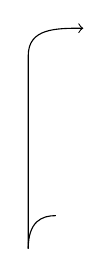
\begin{tikzpicture}[x=0.35cm,y=0.35cm]
\draw[->] (0,0) -- (0,7) .. controls (0,8) and (1,8) .. (2,8);
\draw (0,0) .. controls (0,1) and (0.5,1.2) .. (1,1.2);
\end{tikzpicture}}}
c) Sections horizontales de $\mathcal T\deleted{\unsure{B_u}}$ au-dessus de $\sigma'$ définies par $D$ ($=D_t+\underline\omega=D_t+\lambda(t)\,dt$, où $\lambda(t)$ satisfait (1), ou en satisfait à \unsure{a)}) : les $s:X^{\mathrm{an}}\longrightarrow\mathbf E^{1\mathrm{an}}_{\mathbf C}=\mathbf C$ tels que $D_s=D$, i.e. (posant $s=s(t)$) est $\frac{ds'}{s'}=-\underline\omega$ ($s'=\frac{ds}{dt}$)
\[
(3)\qquad\frac{s''}{s'}=-\lambda(t)\qquad s'=\frac{ds}{dt},\quad s''=\frac{ds'}{dt}.
\]
\unsure{On passe de c) à b)} par $\varphi=ds=s'\,dt$, i.e. $\boxed{\alpha=s'\deleted{\unsure{dt}}}$.

\[
2\left(\unsure{\frac{s''}{s'}|-\frac{s''}{s'}}\right)'+\left(-\frac{s''}{s'}\right)^2=\deleted{\unsure{\bar\omega_2}}\mu(t)
\]
i.e.
\[
-2\frac{s'''s'-s''^2}{s'^2}+\frac{s''^2}{s'^2}\ \deleted{\unsure{=}}\ \mu
\]
\[
\frac{3s''^2-2s's'''}{s'^2}=-2\frac{s'''}{s'}+3\left(\frac{s''}{s'}\right)^2.
\]
\deleted{$\unsure{\lambda'-2\lambda^2}=\mu(t)$}
\[
(4)\qquad\boxed{G_t(s)\overset{\mathrm{d\acute ef}}{=}-2\frac{s'''}{s'}+3\left(\frac{s''}{s'}\right)^2=\mu(t)}
\]
où $s'=\frac{ds}{dt}$, $s''=\frac{ds'}{dt}$, $s'''=\frac{ds''}{dt}$.

Passage de d) à c) : $s\longmapsto(\deleted{\unsure{ds}},\lambda:=-\frac{s''}{s'})$

\unsure{---} d) à b) $s\longmapsto(\alpha=s',\lambda=-\frac{s''}{s'})$

\unsure{---} d) à a) $s\longmapsto\lambda:=-\frac{s''}{s'}$.

\uline{NB} La propriété essentielle de l'expression différentielle $G_t(s)=-2\frac{s'''}{s'}+3(\frac{s''}{s'})^2$ \deleted{\unsure{est}} (\deleted{$=\frac{D_s-D_t}{dt^2}$} ($=\frac{c_{D_s}-c_{D_t}}{dt^2}$)) est son invariance par le groupe homographique :

si \deleted{$\unsure{\widetilde s=s}$}
\[
\widetilde s=\frac{as+b}{cs+d}\qquad a,b,c,d\ \text{constantes},
\]
alors $G_t(\widetilde s)=G_t(s)$ \unsure{\ldots}. De plus, si $\widetilde t$ est un autre uniformisant, on aura
\[
G_{\widetilde t}(s)=G_t(s)\deleted{\unsure{\cdot}}\,\widetilde t'^2.
\]

\uline{Pb} Soit $X$ courbe alg. complète sur $\mathbf C$, $t$ un uniformisant sur un ouvert $U$ de $X$, i.e. application étale $t:U\longrightarrow\mathbf E^1_{\mathbf C}$. Il existe alors une unique section $\mu$ de $\mathcal O_U$ ayant la propriété suivante : Considérons l'équation \uline{alg.} différentielle sur $U^{\mathrm{an}}$, en la fonction analytique inconnue $s:U\longrightarrow\mathbf E^1_{\mathbf C}$
\[
G_t(s)\overset{\mathrm{d\acute ef}}{=}-2\frac{\unsure{s'''|s''''}}{s'}+3\left(\frac{s''}{s'}\right)^2=\mu(t).
\]
Alors les solutions de cette équation, sur $U$
\scanpage{115}
% archive foliation: 114
ouvert \inserted{$V$} de $U^{\mathrm{an}}$, sont des restrictions à $V$ de fonctions \inserted{\unsure{multiformes}} uniformisantes sur $X^{\mathrm{an}}$ (et on \unsure{trouve} \inserted{ainsi} loc. exactement toutes les fonctions uniformisantes).

\uline{Corollaire} Si $X$ n'est pas complète, \unsure{\ldots} le $=$ énoncé avec la seule \unsure{Diff.} que $\mu(t)$ est seulement une section \uline{analytique} de $\mathcal O_U$. \deleted{\unsure{Pouvons nous la}} \inserted{Est-elle} algébrique ? Premiers cas classiques : $X=\mathbf P^1_{\mathbf C}-\text{trois pts}$, ou $X=\text{courbe elliptique}$ moins \uline{un point}.

\uline{Autre question} Quand $X$ (supposons compact disons) varie avec un paramètre \uline{algébrique} parcourant une variété algébrique $S$, i.e. \unsure{\ldots} $X\longrightarrow S$, \unsure{ça donne} comme $\mu$ des fonctions analytiques sur un ouvert de $X$, algébriques sur les fibres. Sont-elles algébriques ? \unsure{Celles-ci, ont elles|Ceci a-t-il} une signification purement algébrique, indépendante de la top. du corps de base $\mathbf C$ -- donc ayant un sens dès que $S$ est un schéma de car nulle ?).
\scanpage{116}
% archive foliation: 115
Soit $X$ une ``courbe analytique'' i.e. espace $\mathbf C$-analytique \uline{régulier} partout de dimension 1. Soit
\[
t:X\longrightarrow\mathbf C
\]
un ``uniformisant'' i.e. \deleted{\unsure{une}} application analytique étale de $X$ dans $\mathbf C=\mathbf E^1(\mathbf C)$, i.e. une section $t$ de $\mathcal O_X$ telle que $dt\in\Gamma(X,\underbrace{\Omega^1_{X/\mathbf C}}_{\underline\omega})$ soit partout $\ne0$ i.e. soit une \uline{base} de $\Omega^1_{X/\mathbf C}$). Soit $s\in\Gamma(X,\mathcal O_X)$ -- \deleted{de préférence} un autre uniformisant, et posons
\[
G(t,s)=\left(-2\frac{s'''}{s'}+3\left(\frac{s''}{s'}\right)^2\right)dt^2\in\Gamma(X,\unsure{\underline\omega^{\otimes2}|\Omega^{\otimes2}})
\]
où $s'=\frac{ds}{dt}$, $s''=\frac{ds'}{dt}$, $s'''=\frac{ds''}{dt}$. On \deleted{\unsure{montre}} vérifie facilement, \deleted{que si $a,b$ sont des constantes, $a\ne0$} \inserted{si $a\in\mathbf C^*$, $b\in\mathbf C$}
\[
(1)\quad\left\{\begin{array}{ll}
G(t,\deleted{\unsure{as}}s+b)=G(t,s)&a)\\
G(t,as)=G(t,s)&b)\\
G(t,\frac1s)=G(t,s)&c)
\end{array}\right.
\]
où, dans la dernière équation, on suppose que $1/s$ est un uniformisant, i.e. $s$ n'a pas de zéros sur $X$. On vérifie de plus que, si $t,s,r$ sont trois uniformisants, on a
\[
(2)\qquad G(t,s)+G(s,r)=G(t,r)
\]
\unsure{Enfin} (3) la formation de $G(t,s)$ commute à la restriction à un ouvert. \deleted{\unsure{En}}

De (1) \inserted{c)} et (3) résulte qu'on peut prolonger l'expression $G(t,s)$ au cas où $s$, au lieu d'être un ``uniformisant'' i.e. un morphisme étale $X\longrightarrow\mathbf E^1(\mathbf C)$, est un morphisme étale
\[
X\longrightarrow\mathbf P^1(\mathbf C)
\]
i.e. une fonction méromorphe n'ayant que des pôles simples, et uniformisante en dehors de ceux-ci -- (dans \inserted{voisinage des} pôles de $s$, on pose $G(t,s)=G(t,1/s)$), et alors \inserted{\unsure{il ne forme plus de} \deleted{\unsure{fonction analytique}} \unsure{où $s$ est holomorphe})} (1) \deleted{devient} reste valable, et \uline{plus généralement}
\[
G\left(t,\frac{as+b}{cs+d}\right)=G(t,s)\qquad
\begin{gathered}a,b,c,d\in\mathbf C\\ad-bc\in\mathbf C^*.\end{gathered}
\]
\scanpage{117}
% archive foliation: 116
D'autre part, faisant $\unsure{t=r|t=s=r}$ dans (2), on trouve
\[
G(t,t)=\deleted{\unsure{G}}0\qquad(t\text{ uniformisant})
\]
et faisant $r=t$, on trouve
\[
G(t,s)+G(s,t)=0,\qquad(s,t\text{ uniformisants})
\]
\inserted{i.e. $G(t,s)=-G(s,t)$}
\deleted{\unsure{donc on} prolonge l'expression $G(t,s)$, définie dans le voisinage par ($t:X\longrightarrow\mathbf E^1(\mathbf C)$, $s\longrightarrow\mathbf P^1(\mathbf C)$), au cas où $t$ peut aussi admettre des pôles.}
\margin{\unsure{ceci permet} \unsure{par (1)} \illegible{2} \unsure{facilement pour} $s,t:X\longrightarrow\mathbf P^1(\mathbf C)$.}
d'où
\[
(1\mathrm{bis})\quad\left\{\begin{array}{l}
G(at,s)=G(t,s)\\
G(t+b,s)=G(t,s)\\
G(\frac1t,s)=G(t,s)\qquad(t,\frac1t\text{ unif}^{\mathrm{ts}})
\end{array}\right.
\]
ce qui permet de faire la $=$ généralisation pour les $t$ que pour les $s$, d'où pour les
\[
s,t:X\longrightarrow\mathbf P^1(\mathbf C)\qquad\text{morphismes étales}
\]
\[
(4)\quad\left\{\begin{array}{l}
G(\frac{at+b}{ct+d},s)=G(t,s)\qquad a,b,c,d\in\mathbf C\text{ avec }ad-bc\in\mathbf C^*\\
\text{en plus de}\\
G(t,\frac{as+b}{cs+d})=G(t,s)\qquad\unsure{''}
\end{array}\right.
\]

\deleted{De plus on a}
Soit $\mathcal P_X$ le faisceau des morphismes \inserted{analytiques} étales
\[
X\longrightarrow\mathbf P^1(\mathbf C),
\]
sur lequel opère le groupe
\[
H=\operatorname{Aut}_{\mathbf C}\mathbf P^1(\mathbf C)\simeq\mathrm{GP}(1)(\mathbf C):=\left\{\left(\begin{matrix}a&b\\c&d\end{matrix}\right)\,\middle|\,ad-bc\in\mathbf C^*\right\}\quad\text{mod. matrices diagonales}.
\]
On a donc défini un morphisme de faisceaux
\[
\underline G:\mathcal P_X\times\mathcal P_X\longrightarrow\deleted{\unsure{\Omega}}\underline\omega_X^{\otimes2}
\]
satisfaisant les deux conditions

I) $G$ invariant par $H\times H$ i.e.
\[
G(gt,g's)=G(t,s)\qquad\text{si }g,g'\in H
\]
II) $G(t,s)+G(s,r)=G(t,r)$

En particulier $G(t,t)=0$, $G(t,s)=-G(s,t)$ \unsure{(pour $s$, pour $t$ fixé)}.

En fait, la théorie des équations différentielles nous donne aisément une réciproque à I), savoir
\scanpage{118}
% archive foliation: 117
III) a) Si $s,t\in\Gamma(U,\mathcal P_X)$, $U$ connexe, \deleted{\unsure{donc}} et $G(t,s)=0$, alors $\exists\deleted{\unsure{unique}}\ g\in H$ tel que $t=g\cdot s$.

b) Pour $t$ fixé, le morphisme
\[
s\longmapsto G(t,s)\qquad \mathcal P_X\longrightarrow\underline\omega_X^{\otimes2}
\]
(qui induit un hom. injectif $\deleted{\unsure{\mathcal P_X/H}}\ H\backslash\mathcal P_X\lhook\joinrel\longrightarrow\underline\omega_X^{\otimes2}$, d'après a)) est \uline{surjectif} (i.e.
\[
H\backslash\mathcal P_X\xrightarrow{\sim}\underline\omega_X^{\otimes2}\qquad s\longmapsto G(t,s)=\left(-2\frac{s'''}{s'}+3\left(\frac{s''}{s'}\right)^2\right)dt^2
\]

D'autre part, grâce à II, on peut donner une forme plus simple et intrinsèque à l'expression $G(t,s)$.

\uline{Proposition} (qui est formelle à partir de (II)) On peut, \inserted{à isomorphisme unique près,} trouver un torseur $\operatorname{Conn}_X$ sous $\underline\omega_X^{\otimes2}$, et un morphisme de faisceaux
\[
t\longmapsto c_t:\quad\mathcal P_X\xrightarrow{c^X}\operatorname{Conn}_X
\]
tels que l'on ait, pour $s,t\in\Gamma(U,\mathcal P_X)$
\[
\boxed{G(t,s)=c_s-c_t}
\]

\margin{!}
Le faisceau $\operatorname{Conn}_X$ est appelé le \uline{faisceau des connexions projectives} (analytiques complexes) sur $X$. Une section dudit est appelé \uline{connexion projective} (analytique) de $X$. Le morphisme $c^X$ est inv. par $H$ et induit par passage au quotient un iso. can.
\[
c^X:H\backslash\mathcal P_X\xrightarrow{\sim}\operatorname{Conn}_X.
\]
Un morphisme étale
\[
f:X'\longrightarrow X
\]
définit des iso.
\[
\mathcal P_{X'}\simeq f^{-1}(\mathcal P_X)\qquad \operatorname{Conn}_{X'}\simeq f^{-1}(\operatorname{Conn}_X)
\]
et on trouve un \deleted{\unsure{même}} diag. comm.
\diagram{\begin{tikzcd}
\mathcal P_{X'}\arrow[r,"c^{X'}"]\arrow[d,"\sim"']&\deleted{\unsure{\mathcal C_{X'}}}\operatorname{Conn}_{X'}\arrow[d,"\sim"]\\
f^{-1}(\mathcal P_{\unsure{X'|X}})\arrow[r,"c^X"']&f^{-1}(\operatorname{Conn}_X)
\end{tikzcd}}
\scanpage{119}
% archive foliation: 118
Notons que si $X_0=\mathbf P^1(\mathbf C)$ \deleted{il y a} le faisceau $H\backslash\mathcal P_{X_0}$ est le faisceau final, \deleted{\unsure{et que}} \deleted{\unsure{il y a}} il y a une conn. projective can. \inserted{$c$} sur $X_0$, savoir $c_t$ pour $t=\operatorname{id}_{X_0}$ ! C'est la seule conn. projective sur $X_0$, car $H^0(X_0,\underline\omega_{X_0}^{\otimes2})=0$ ($\underline\omega$ est de degré $-2$, donc $\underline\omega^{\otimes2}$ de degré $-4$ !).

Revenant au cas d'un $X$ général, on voit donc que
\[
c_t=t^*(c)=\text{image inverse par }t\text{ de la conn. projective can. }c
\]
(l'unique conn. proj.) sur $\mathbf P^1(\mathbf C)$.
\deleted{\unsure{c}}

\uline{Extension à la géom. alg.} Soit maintenant $X$ schéma form$^{\mathrm t}$. lisse de dim \inserted{diff} relative 1 sur un schéma $S$. Si \deleted{$t,s:$}
\[
t,s:X\longrightarrow\mathbf E^1_S
\]
sont étales \inserted{\unsure{topologiques}}, on définit comme plus haut
\[
G(t,s)\in\Gamma(X,\underbrace{(\Omega^1_{X/S})^{\otimes2}}_{\underline\omega^{\otimes2}}),
\]
et on vérifie bien sûr (1) et (2) par le $=$ calcul que dans le cas analytique, ce qui permet d'étendre $G(t,s)$ au cas de morphismes \uline{étales}
\[
t,s:X\longrightarrow\mathbf P^1_S
\]
\deleted{\unsure{topologiques}}, de façon à satisfaire encore \deleted{$t,s:X\longrightarrow$}

(posant $H_S=\underline{\operatorname{Aut}}_S(\mathbf P^1_S)$)
\[
G(gt,g's)=G(t,s)\qquad(g,g'\in\Gamma(S,H))
\]
et à définir ainsi, si $\mathcal P_{X/S}$ est le faisceau \inserted{(ét)} des morphismes étales $X\longrightarrow\mathbf P^1_S$, \deleted{\unsure{défini par}} \inserted{un morphisme can.}
\[
G:\mathcal P_{X/S}\times\mathcal P_{X/S}\longrightarrow\underline\omega_{X/S}^{\otimes2}.
\]
\margin{\unsure{au lieu de diff. principales parler plutôt de diff. uniques} jusqu'à l'ordre 3, i.e. \unsure{que} $\unsure{P^3_{X/S}}$ \unsure{$\simeq\operatorname{Sym}(\underline\omega_{X/S})$} \unsure{en degrés} $\le3$.}
\scanpage{120}
% archive foliation: 119
\uline{Invariant} sous l'action de $f^{-1}(H_S)$ i.e. telle que
\[
G(g\cdot s,g'\cdot t)=G(s,t)\quad\text{si}\quad
\left\{\begin{array}{l}s,t\in\Gamma(U,\mathcal P_X)\\g,g'\in\Gamma(V,H_V)\end{array}\right.
\]
\diagram{\begin{tikzcd}
U\arrow[r,"\text{ét}"]\arrow[d]&X\arrow[d,"f"]\\
V\arrow[r,"\text{ét}"']&S
\arrow[ul,phantom,"\text{comm.}"]
\end{tikzcd}}
et satisfaisant
\[
G(s,t)+G(t,r)=G(s,r).
\]
Cela permet donc de définir le faisceau \inserted{$\operatorname{Conn}_{X/S}$} (ét) des conn. projectives sur $X$ rel. à $S$, qui est un torseur sous $\underline\omega_{X/S}^{\otimes2}$, et d'interpréter $G(t,s)$ à l'aide d'un morphisme canonique
\[
c^X:\mathcal P_{X/S}\longrightarrow\operatorname{Conn}_{X/S}
\]
par
\[
G(t,s)=c^X_{\unsure{t}}(s)-c^X(t).
\]

Enfin, par construction la formation de $\mathcal P_{X/S}$, $\operatorname{Conn}_{X/S}$ et $c^X$ commute à la loc. étale. Cela permet d'interpréter encore
\[
c^X(t)=t^*(c)
\]
où $c$ est l'unique connexion sur $\mathbf P^1_S$.

Plus gén., pour un fibré en droites projectives $X_0$ sur $S$, il y a une unique conn. proj. $c_{X_0}$ sur $X_0$, et si $t,s:X\longrightarrow X_0$ sont étales on peut définir
\[
G(t,s)=c_{(s)}-c_{(t)}=s^*(c_{X_0})-t^*(c_{X_0})
\]
satisfaisant aux conditions analogues à celles du cas $X_0=\mathbf P^1_S$, que le lecteur (bis) \unsure{énoncera}.
\scanpage{121}
% archive foliation: 120
Si $S$ est de car. 0, alors $X$ est \inserted{(lisse/$S$ ??)} à fibres géom. connexes non vides, \unsure{on peut énoncer que} pour $s,t:X\longrightarrow X_0$ (fibré en droites projectives sur $S$) étales, tels que $G(t,s)=0$ i.e. $t^*(c_{X_0})=s^*(c_{X_0})$, il existe
\[
g\in\operatorname{Aut}(X_0)
\]
tel que $s=g\circ t$.
\margin{\uline{à vérifier !}}
Donc, pour $t$ fixé, $s$ variable, le morphisme
\[
f^{-1}(H_S)\backslash\mathcal P_X\longrightarrow\deleted{\unsure{\Omega}}\underline\omega_{X/S}^{\otimes2}\qquad s\longmapsto G(t,s)
\]
est \uline{injectif}, ou encore (intrinsèquement) le morphisme
\[
H\backslash\mathcal P_X\xrightarrow{c^X}\operatorname{Conn}_{X/S}
\]
défini par passage au quotient par $c^X$, est \uline{injectif}. \deleted{\unsure{H\backslash}} Mais bien sûr ces deux morphismes ne sont plus \deleted{bijectifs} surjectifs. Une conn. \unsure{affine|projective} qui est \deleted{\unsure{contenue}} dans l'image de $H\backslash\mathcal P_X$ est dite ``intégrable par fonctions algébriques''.

Si $S$ est de car. pos., alors l'injectivité n'est pas non plus valable non plus. Introduisons $X^{(p/S)}$ et
\diagram{\begin{tikzcd}
X\arrow[rr,"F_X"]\arrow[dr]&&X^{p/S}\arrow[dl]\\
&S&
\end{tikzcd}} (Frobenius)
On trouve que le \deleted{\unsure{groupe $H_{X/S}$}} \inserted{$H(X^{p/S})$}, opère \unsure{\ldots} \uline{de façon évidente}, sur $\deleted{\unsure{\mathcal P_X}}\ \Gamma(X,\mathcal P_X)=\operatorname{Ét}_S(X,\mathbf P^1_S)$, laisse invariant l'expression $G(t,s)$, et le même \unsure{argumentation opère}, i.e. d'où encore
\[
F_X^{-1}(H_{X^{p/S}})\backslash\mathcal P_X\lhook\joinrel\longrightarrow\operatorname{Conn}_{X/S}.
\]
\margin{\unsure{$2$ et $3$ sont inversibles, en car. $p>3$ !} Cf plus bas !}

Introduisons (\unsure{si $s,t$ sont} \deleted{deux} \inserted{\unsure{deux}} uniformisants) l'opérateur
\[
D_t^{(n)}f=\frac1{n!}\frac{d^nf}{dt^n}
\]
(qui a un sens sans restriction de car. nulle, dès que $X/S$ est diff. lisse de \deleted{\unsure{dim}} \inserted{dim rel.} ($=1$)), on trouve alors que (pour tout uniformisant)
\[
G(t,s)=12\left(-\frac{D_t^{(3)}s}{D_t^{(1)}s}+\left(\frac{D_t^{(2)}s}{D_t^{(1)}s}\right)^2\right)=12G_0(t,s)
\]
où
\[
G_0(t,s)=-\frac{D_t^{(3)}s}{\unsure{D_t^{(1)}}s}+\left(\frac{D_t^{(2)}s}{\unsure{D_t^{(1)}}s}\right)^2.
\]
Cela montre que si $12\cdot1_S\deleted{\unsure{\ne}}=0$, alors toutes les connexions projectives de la forme $c_t$ sont \uline{égales}, donc il y a une conn. proj. canonique sur $X$ rel. à $S$, à laquelle on peut référer toutes les autres. Cela montre aussi (sans restriction de car. telle $12\cdot1_S=0$ !) que le torseur $\deleted{\unsure{\mathcal T}}\operatorname{Conn}_{X/S}$ est déduit, moyennant le chgt de groupe d'op.
\[
\underline\omega_{X/S}^{\otimes2}\xrightarrow{12\cdot\mathrm{id}}\underline\omega_{X/S}^{\otimes2},
\]
d'un torseur plus fin $\operatorname{Conn}_{0\,X/S}$ \inserted{sous $\underline\omega_{X/S}^{\otimes2}$}, avec un morphisme
\[
\mathcal P_{X/S}\xrightarrow{c_0^X}\operatorname{Conn}_{0\,X/S}
\]
tel que
\[
c_0^X(s)-c_0^X(t)=G_0(t,s).
\]
Bien entendu, les assertions plus haut sur l'expression $G(t,s)$ et les connexions
\scanpage{122}
% archive foliation: 121
\inserted{$\operatorname{Conn}_{X/S}$ et de}
\[
H\backslash\mathcal P_{X/S}\longrightarrow\operatorname{Conn}_{X/S}
\]
s'étendent à $G_0(t,s)$ et à
\[
H\backslash\mathcal P_{X/S}\longleftrightarrow\operatorname{Conn}_{0\,X/S},
\]
les premières se déduisant des secondes de façon évidente, compte tenu de l'hom. can.
\[
\operatorname{Conn}_{0\,X/S}\longrightarrow\operatorname{Conn}_{X/S}
\]
compatible avec l'hom.
\[
\underline\omega_{X/S}^{\otimes2}\xrightarrow{12\cdot\mathrm{id}}\underline\omega_{X/S}^{\otimes2}
\]
sur les Groupes d'opérateurs. (On \deleted{posera} \inserted{écrira} parfois $c_0^X(t)=\frac1{12}c^X(t)$ \ldots)

On peut espérer que si $S$ de car. $p>0$ et si $\mathcal O'_X$ est le ss-faisceau de $\mathcal O_X$ \deleted{défini par} \inserted{\unsure{à qui s'appliquent}} les conditions $D_t^{(i)}f=0$ ($i\le3$)
\[
H_{X^{(p/S)}}\backslash\mathcal P_{X/S}\lhook\joinrel\longrightarrow\operatorname{Conn}_{0\,X/S}
\]
soit \uline{injectif}, i.e. qu'on a
\margin{$\mathcal O'_{X/S}$ est $\mathcal O_{X/S}^{(p)}$ si $p\ne2,3$, sinon c'est $\mathcal O_{X/S}^{(p^2)}$.}
\margin{\uline{OK}}

\uline{Proposition} \deleted{\unsure{Non vérifiée}} $A$ anneau de car. $p>0$, \inserted{local (plus gén. \unsure{avec} $\operatorname{Pic}(A)=0$)}, $\alpha\in A$, $B=A[T]/(T^p-\alpha)$, $t\in B$ la classe de $\deleted{B}T$ dans $B$ (donc $t^p=\alpha$), $\unsure{\forall|\exists}\ s\in B$, donc
\[
s=a_0+a_1t+\cdots+a_{p-1}t^{p-1}\qquad a_i\in A\ (0\le i\le p-1).
\]
\margin{car. $p\ne2,3$ (\unsure{hypothèse provisoire})}
Posons
\deleted{$D_t^{(j)}s=\sum_{j\le i\le p-1}a_i\binom ij t^{i-j}$},
\inserted{$D_t^1s:=(ds)/(dt)$, $D_t^{(i)}s:=\frac1{i!}(D_t^1)^is$ si $1\le i\le3$, et}
\[
\deleted{\unsure{G_0}}\ c_0(s)=-\frac{D_t^{(\unsure{3|2})}s}{D_t^{(1)}s}+\left(\frac{D_t^{(2)}s}{D_t^{(1)}s}\right)^2\qquad\text{si }D_t^{(1)}s\in B^*.
\]
Supposons $c_0(s)=0$ i.e.
\[
(D^{(3)}s)^2=(D^{(1)}s)(D^{\unsure{(2)|(3)}}s).
\]
Alors $\exists a,b,c,d\in A$ \inserted{(uniques à \unsure{transformation} \uline{diagonale})} avec $ad-bc=1$, tels que
\[
s=\frac{at+b}{ct+d}\qquad\text{i.e.}\quad s(ct+d)=at+b
\]
\scanpage{123}
% archive foliation: 122
OPS \deleted{\unsure{quitte}} par changement $\unsure{\alpha\in}\deleted{\unsure{A}}A^p$, puis $\alpha\unsure{=|\ne}0\deleted{\unsure{\alpha}}$. \deleted{\unsure{alors}} $t\in\unsure{\mathfrak r B|\sqrt{0_B}}$, donc
\[
D^{(1)}s=a_1+a_2t+\cdots\equiv a_1\ (\unsure{\mathfrak r B}),
\]
donc $D^{(1)}s\in B^*\Longleftrightarrow a_1\in A^*$. OPS, quitte à remplacer $s$ par $a_1^{-1}(s-a_0)$, que $s=t+a_2t^2+\cdots+a_{p-1}t^{p-1}$ puis, quitte à faire encore un chgt de variable \deleted{\unsure{et}}
\[
s'=\frac{s}{1+a_2s}=\deleted{\unsure{\frac1{1+a_2s^{-1}}}}=\deleted{\unsure{s}}\sum_{n\ge0}\inserted{(-1)^n}a_2^n s^{n+1}
\]
$=s\unsure{-|+}a_2s^2+\cdots\equiv t\bmod t^3$ donc $s$ de la forme
\[
s=t+\text{termes d'ordre }\ge3.
\]
\deleted{Alors} À prouver que, dans ces conditions, la condition
\[
c_0(s)=0\Longrightarrow s=t.
\]
\deleted{\unsure{Si on a}} Il suffit de prouver que si
\[
s=t+at^d+\cdots\quad(\text{termes d'ordre }\ge d+1)
\]
où $\deleted{d\ge3}\inserted{3\le d\le p-1}$, alors $a=0$.
\[
D^{(3)}s\equiv a\binom d3t^{d-3}\bmod(t^{d-2})
\]
\[
D^{(2)}s\equiv a\binom d2t^{d-2}\bmod(t^{d-1})\quad\text{et a fortiori mod }t^{d-2}
\]
\[
D^{(1)}s\equiv1\deleted{+ad\,t^{d-1}}\bmod(t^{d-1})\quad\text{et a fort. mod }t^{d-2}
\]
\[
D^{(3)}s\,D^{(1)}s\equiv a\binom d3t^{d-3}\deleted{+a^2d\binom d3t^{2d-4}}\quad\bmod t^{d-2}
\]
\[
(D^{(2)}s)^2\equiv0\quad\bmod t^{d-2}
\]
donc $a\binom d3t^{d-3}\equiv0\quad\bmod t^{d-2}$

donc $a\binom d3=0$ dans $A$,

i.e. $\dfrac{d(d-1)(d-2)}6\,a=0$ dans $A$

or 6 inv. dans $A$, et aussi $d(d-1)(d-2)$ car $3\le d\le p-1$ et $A$ de car. $p>3$, donc $a=0$ OK.
\scanpage{124}
% archive foliation: 123
\uline{Cas car. 2 ou 3} --- Ici il faut supposer
\[ B=A[T]/(T^{p^2}-\alpha), \]
sinon l'énoncé (modulo rectification de la \deleted{définition}\inserted{description} des $D_t^{(i)}\ldots$) du résultat sur \unsure{formes d'hog. comme}, et la réduction au cas $\alpha=0$, $s\equiv t\ (t^3B)$, est comme dessus. Il faut prouver que $s=t$, donc si
\[s=t+at^d\qquad(3\leq d\leq\deleted{\unsure{p}}p^2-1)\]
alors $a=0$. On trouve comme tantôt
\[a\binom d3=0\quad\text{i.e.}\quad a\underbrace{c_{3,d-3}}_{\text{coeff. binom.}}=0,\]
d'autre part $c_{\unsure{3|2},d-3}\in\mathbb F_p^*$ ssi. \deleted{$d\text{ et }d-3$} pour
\[
\begin{gathered}
d-3=d_0+d_1p\\
\unsure{3}=d'_0+d'_1p
\end{gathered}
\qquad(0\leq d_0,d_1,d'_0,d'_1\leq p-1)
\]
on a $d_0+d'_0\leq p-1$, $d_1+d'_1\leq p-1$.

1) Cas car. $p=2$, \deleted{$\unsure{d-d'_0}=\unsure{1}(d_0-1)+(d_1-1)p$}
\deleted{Car $d_0,d_1\geq1$ \unsure{le cas favorable est celui}.}
Car l'\uline{unique} est $d=3$ \deleted{$\unsure{d\leq p}$}.
\deleted{\unsure{donc}}
\[c_{3,0}=1\quad\Longrightarrow a=0\qquad\text{OK}\]
\deleted{\unsure{d_0=d_1=0}}

2) \uline{Cas $p=3$}. \deleted{\unsure{pour}}
\deleted{Si $d_1\ne0$ i.e. $d_1\geq1$,
\[
d-3=d-p=d_0+(d_1-1)p,\quad\text{et}
\]
\[
c_{d,d-3}=c_{d_0,d_0}c_{d_1,d_1-1}\quad\text{dans }\mathbb F_p
\]
\[
\in\mathbb F_p^*\quad\text{ssi}\quad
\begin{gathered}2d_0\leq p-1=2.\\2d_1-1\leq p-1=2.\end{gathered}
\]
i.e. $d_1=1$, $d_0=0$ ou $1$, donc cas qui échappent
\[
\text{c) }\textcircled{$d_1=0$},\quad\text{a) }d_1=2.\qquad\text{b) }d_1=1,\ d_0=2.
\]
\unsure{Le cas} $d_1=0$ est au fond favorable, car alors $3\leq d\leq p-1$ donc $c_{d,d-3}$}

\[
d-3=d_0+d_1p\qquad0\leq d_0,d_1\leq2
\]
\margin{et comme $0\leq d-3\leq5$ (car \deleted{$d$} $3\leq d\leq p^2-1=8$)}
\deleted{$0\leq d_1\leq\unsure{3}$}
\[\inserted{d_1\leq1}\]
\[3=0+1\times p\]
La condition $c_{3,d-3}\in\mathbb F_p^*$ signifie ici
\[
d_1+1\leq p-1\quad\text{i.e.}\quad\deleted{\unsure{p}}\ d_1+1\leq2\quad\text{i.e.}\quad d_1\leq1,
\]
qui est vérifiée. On gagne encore !
\figure{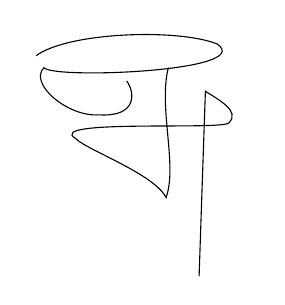
\begin{tikzpicture}[x=1cm,y=1cm]
\draw (0,2.8) .. controls (0.4,3.1) and (1.8,3.15) .. (2.3,2.95) .. controls (2.8,2.6) and (0.2,2.5) .. (0.1,2.65) .. controls (-0.1,2.45) and (0.4,2.02) .. (0.8,2.05) .. controls (1.3,2.02) and (1.25,2.35) .. (1.15,2.48);
\draw (1.68,2.65) .. controls (1.55,2.15) and (1.8,1.4) .. (1.65,1.0) .. controls (1.5,1.3) and (0.65,1.6) .. (0.5,1.75) .. controls (0.1,2.0) and (2.4,1.85) .. (2.45,1.95) .. controls (2.6,2.1) and (2.3,2.25) .. (2.15,2.35) -- (2.07,0);
\end{tikzpicture}}
\scanpage{126}
% archive foliation: 125
Soit $P$ une droite projective sur $\mathbb C$. Un ouvert non vide $D\subset P^{\mathrm{an}}$ est dit ``\uline{homogène}'' si le \inserted{sous-}groupe $G$ de $\operatorname{Aut}(P)\xrightarrow{\sim}\operatorname{Aut}(P^{\mathrm{an}})$ $(\simeq\mathrm{GP}(1)_{\mathbb C})$ agit homogènement sur $D$. Si $D$ est homogène et $g\in\operatorname{Aut}(P)$, $g(D)$ est homogène et a comme groupe de stabilité $\operatorname{int}(g).G$.

Le ``théorème d'uniformisation'' nous donne

\uline{Th. (classique) 1.}

a) Il y a exactement trois classes (à op. près de $\operatorname{Aut}(P)$) de domaines homogènes dans $P$, savoir
\[
\begin{aligned}
1^\circ)\quad&D=P\\
2^\circ)\quad&D=P-\{x\}\qquad\text{où }x\in P
\end{aligned}
\]
$3^\circ)$ $D$ un disque ouvert [pour une métrique \inserted{riemannienne} (invariante) sur $\unsure{X|P}$ --- NB les métriques \inserted{invariantes} (\deleted{sont} toutes multiples scalaires de l'une d'elles, et les disques ouverts pour \deleted{une}\inserted{telle} métrique sont \unsure{indépendants} du choix de celle-ci]

b) Pour $D$ domaine homogène dans $\unsure{X|P}$, $G\subset\operatorname{Aut}(P)$ son stabilisateur, l'application $G\longrightarrow\operatorname{Aut}(D)$ est un iso. De plus, $D$ est connexe et simplement connexe.

c) Le foncteur $(P,D)\longmapsto D$, de la catégorie \inserted{(pour iso)} des couples $(P,D)$, $P$ droite projective et $D$ domaine homogène de $P$, dans la catégorie \inserted{(pour iso)} des espaces $\mathbb C$-analytiques réguliers de dim 1 connexes et simplement connexes, est une équivalence de catégories.

\uline{Corollaire} Les groupes $G$ de stabilité d'un domaine homogène $D$ de $P$ sont respectivement
\[
\begin{aligned}
1)\quad&\operatorname{Aut}(P)\quad(\simeq\mathrm{GP}(1,\mathbb C))\\
2)\quad&\operatorname{Aut}(E^1)\quad(\simeq\operatorname{Aff}(1,\mathbb C))\\
3)\quad&\simeq\mathrm{GP}(1,\mathbb R)\simeq\mathrm{GL}(2,\mathbb R)/\mathbb R^*\simeq\mathrm{SL}(2,\mathbb R)/\mu_2(\mathbb R)
\end{aligned}
\]
(On notera la différence entre $1^\circ)$ et $2^\circ)$ d'une part, où on trouve (des groupes analytiques associés à) un groupe algébrique sur $\mathbb C$, et le cas $3^\circ$
\scanpage{127}
% archive foliation: 126
 où on trouve \deleted{un groupe algébrique \uline{réel} $\mathrm{GP}(1)_{\mathbb R}$}\inserted{le groupe des points réels $\mathrm{GP}(1,\mathbb R)$} --- qui en fait est une forme réelle du $\mathrm{GP}(1)_{\mathbb C}$, \deleted{\unsure{donnant un stabilisateur}}\inserted{\unsure{d'ailleurs il se trouve}} qu'le \deleted{choix d'une}\inserted{\unsure{correspond}} \deleted{forme} biunivoque entre

$\alpha)$ choix d'une \deleted{forme réelle}\inserted{descente du corps de base de $\mathbb C$ à $\mathbb R$} dans le groupe alg. \deleted{$\unsure{\mathrm{GP}_{\mathbb C}}$} $\operatorname{Aut}_{\mathbb C}P$

$\beta)$ choix d'une descente du corps de base de $\mathbb C$ à $\mathbb R$ dans l'algèbre de Lie complexe
\[
\operatorname{Lie}\operatorname{Aut}_{\mathbb C}P=\mathrm H^0(P,\mathcal T_{P/\mathbb C})\simeq\mathrm H^0(P,\Omega^{-1}_{P/\mathbb C})
\]
$\gamma)$ choix d'un domaine homogène de type $3^\circ$ (i.e. non algébrique) dans $P$, à polarité près (la polaire de $D$ est $\complement\overline D$).

\margin{$\delta)$ choix d'un \unsure{géodésique non ponctuel} ($=$ cercle) dans $P$}
La relation entre $\alpha)$ et $\beta)$ claire, celle entre \unsure{$\delta)$|$\alpha)$} et $\gamma)$ est la suivante : À une \deleted{\unsure{déforme}} projective réelle $\inserted{P_{\mathbb R}}$, on associe l'ens. de ses pts réels, qui est un ``cercle'' dans $P_{\mathbb R}(\mathbb C)=P(\mathbb C)$ $(P=P_{\mathbb R}\otimes_{\mathbb R}\mathbb C)$, et on prend les deux composantes connexes de $P_{\mathbb R}(\mathbb C)-P_{\mathbb R}(\mathbb R)\ldots$ Notons que l'inversion, par un cercle $P_{\mathbb R}(\mathbb R)$

\uline{Scholie} On a un foncteur $\inserted{P}$ de la catégorie des courbes analytiques non sing. connexes et simplement connexes $\inserted{X}$ vers la catégorie des droites projectives complexes, et une immersion fonctorielle
\[X\lhook\joinrel\xrightarrow{i_X}P(X)(\mathbb C)\]
faisant de $X$ un domaine \unsure{strict.} hom. de $P(X)$.
Un tel foncteur est unique (à iso unique près respectant $i:\operatorname{id}\longrightarrow P(-)(\mathbb C)$).

Soit maintenant $X$ une courbe analytique non singulière. Pour tt pt $x\in X$, soit $\widetilde X(x)$ le rev. universel de $X$ en $x$. C'est un espace analytique simplement connexe, et quand $x$ varie, on reçoit un système local (foncteur du groupoïde fondamental $\Pi(X)$ de $X$) à valeurs les $\widetilde X(x)$ (considérés comme objets de la cat des \deleted{esp.}\inserted{courbes} analytiques connexes et simplement connexes, \unsure{munis par pt donné}). Le système des projections
\[\widetilde X(x)\longrightarrow X=X(x)\]
est un hom. de systèmes locaux d'espaces analytiques. On lui associe donc toujours un hom. d'espaces analytiques sur $X$
\diagram{\begin{tikzcd}
\widetilde X\arrow[r]\arrow[dr]&X\times X\arrow[d,"\operatorname{pr}_2"]\\
&X
\end{tikzcd}}
munis de connexions intégrables (au sens strict : il y a transport parallèle\ldots)
L'hom. est compatible avec les connexions, et transforme la section marquée $\sigma:x\mapsto\widetilde x$ de $\widetilde X$ en la section diagonale de $X$ (d'où on conclut que $\sigma$ est analytique).

Cette construction marche pour tt espace analytique. Mais utilisant le fait que $\deleted{X}$ est une courbe non sing., donc les $\widetilde X(x)$ sont des courbes non sing. conn. et simplement connexes, on trouve que le système local des $\widetilde X(x)$ donne naissance au système local des $P(\widetilde X(x))(\mathbb C)$, d'où un \uline{fibré projectif canonique}, $\mathcal P$, sur
\scanpage{128}
% archive foliation: 127
$X$, $P_X$, avec une \deleted{\unsure{immersion}}\inserted{connexion} intégrable, et une immersion \inserted{de $X$-espaces} (respectant les connexions)
\diagram{\begin{tikzcd}
\widetilde X\arrow[r,phantom,"\subset"]\arrow[dr,dash]&P_X\arrow[d,dash]\\
&X
\end{tikzcd}}
Comme $\widetilde X$ est muni d'une section marquée analytique, $P_X$ a une section marquée analytique.

Donc

\uline{Théorème 2} Pour $X$ courbe analytique \deleted{\unsure{décrite}}\inserted{non sing.}, on peut trouver, de façon unique :
(à iso unique près),
\[
\left\{\begin{aligned}
\text{a)}\quad&\text{Un fibré analytique }P_X\text{ sur }X\text{ en droites projectives}\\
\text{b)}\quad&\text{Une connexion (intégrable) sur }P_X\ (\text{rel : }X/\mathbb C)\\
\text{c)}\quad&\text{Une section }\sigma\text{ de }P_X\text{ sur }X\\
\text{d)}\quad&\text{Un ouvert }\widetilde X\text{ de }P_X\text{ contenant }\sigma(X)\\
\text{e)}\quad&\text{Un hom. de }X\text{-espaces analytiques }\widetilde X\xrightarrow{p}X_X=X\times X
\end{aligned}\right.
\]
\margin{Car b) c) impliquent déjà \unsure{un germe $\widetilde p$ d'hom. anal. possédant des solutions} le long de $\sigma$ \unsure{supposée} (dire que $\sigma$ est nulle part stationnaire signifie que $p$ est un iso le long de $\sigma$) et on fait \unsure{alors du} prolongement analytique de ce germe ($\widetilde p\ldots$) cf \unsure{explication} plus bas.}
tels que
\[
\begin{aligned}
1^\circ)\quad&p\circ\sigma=\Delta_X\quad(\text{section diagonale})\\
2^\circ)\quad&\forall x\in X,\quad p_x:\widetilde X_x\longrightarrow(X_X)_x=X
\end{aligned}
\]
fait de $\widetilde X_x$ un rev. universel de $\inserted{\text{la comp. connexe de }x\text{ dans }}X$ (i.e. c'est un rev. de $X$, connexe et simplement connexe)

$3^\circ)$ $p$ est compatible avec les connexions

$4^\circ)$ $\forall x\in X$, $\widetilde X_x\subset(P_X)_x$ est un domaine homogène de $(P_X)_x$.

\margin{Les données \inserted{d/ et} e) satisfaisant $1^\circ\ 2^\circ\ 3^\circ$ sont déjà \uline{canoniquement} \unsure{définies par} a) b) c) \unsure{avec des}\ \uline{\unsure{restrictions}} dessus.}
\scanpage{129}
% archive foliation: 128
Supposons $X$ connexe et distinguons les 3 cas, suivant le type d'isomorphie du rev. universel de $X$.

$1^\circ)$ Cas $S^2=P^1_{\mathbb C}(\mathbb C)$. Alors $X\unsure{\simeq}P^1_{\mathbb C}$ est lui-même une droite projective (car, sur une droite projective, tout autom. analytique --- et \unsure{on donne aucune condition} --- a un pt fixe au moins\ldots), $\widetilde X=X\times X\inserted{=P_X}$ avec connexion triviale, $p$ est l'identité.

$2^\circ)$ Cas $E^1(\mathbb C)=\mathbb C$. Alors $X$ est soit \deleted{isomorphe} une courbe elliptique (cas $X$ comp. rég.) soit isomorphe à $\mathbb C$, ou à $\mathbb C^*$ (cela provient du fait que les \deleted{sous-groupes discrets}\inserted{autom. sans pt. fixe} de \deleted{\unsure{\mathbb R}\text{ les}} $E^1_{\mathbb C}$, \inserted{analytiques comme de $E^1_{\mathbb C}$, c'est kifkif}) \deleted{de $\operatorname{Aff}(1,\mathbb C)\simeq\mathbb C^*\cdot\mathbb C$ (\unsure{pour des raisons de comp.})} \inserted{sont des translations}, et les sous-groupes discrets \deleted{\unsure{contenus dans le sous-groupe des translations}} du groupe des translations $\mathbb C$ sont de rang $0$ (point $\mathbb C$), ou $1$ (point $\mathbb C^*$) ou $2$ (point courbe elliptique). On voit que $X$ est encore can. muni d'une structure algébrique (tout autom. analytique d'une courbe elliptique, ou d'un $E^1_{\mathbb C}$, ou de $\mathbb G_{m\mathbb C}$, étant algébrique).

\margin{La cat. (pour iso) des courbes analytiques du type $2^\circ$ est équivalente (par le foncteur $X\mapsto X^{\mathrm{an}}$) à la catégorie des torseurs sous \deleted{\unsure{groupes linéaires}} des groupes algébriques sur $\mathbb C$ connexes de dim 1 (\unsure{comm. $\Rightarrow$ donc}, $\mathbb G_a$, $\mathbb G_m$, ou une VA de dim 1), et \unsure{can. on peut munir une telle courbe d'une structure de torseur sur $\mathbb C$}, un $\mathbb G_a$-torseur, un $\mathbb G_m$-torseur, ou une VA de dim 1).}

Ici $\widetilde X=P_X-\sigma'$, où $\sigma'$ est une \uline{section horizontale} de $P_X$ ; donc, \deleted{$P_X$ est}\inserted{$P_X$ étant} muni des deux sections analytiques $\sigma,\sigma'$ disjointes, on peut considérer $P_X$ comme clôture projective d'un fibré vectoriel analytique $V$, qui n'est autre que $\widetilde X$ comme esp. analytique sur $X$ --- mais \deleted{\unsure{muni au fond d'un fibré}}\inserted{pourvu d'une structure vectorielle}. On observera que la connexion de $V$ \deleted{\unsure{ne lui}} n'honore pas la structure vectorielle. Mais on peut
\scanpage{130}
% archive foliation: 129
écrire $V=\mathbb V(\omega_\sigma)$, $\omega_\sigma$ étant le fibré conormal le long de la section $\sigma$, qui est aussi isom. au fibré conormal de $X_X$ le long de la section diagonale, donc
\[
V=\mathbb V(\underbrace{\Omega^1_{X/\mathbb C}}_{\omega_{X/\mathbb C}})=\mathbb W(\underbrace{t_{X/\mathbb C}}_{\text{fibré tangent}}).
\]
Donc $\widetilde X$ s'identifie au fibré tangent à $X$, $\sigma$ à la section nulle, $P_X$ à la clôture projective de $\widetilde X=\mathbb W(t_{X/\mathbb C})$. La connexion \deleted{intégrable}\inserted{plate} canonique de $P_X$ est associée à une connexion de $\widetilde X$ \uline{considéré comme fibré en droites affines}, i.e. une connex. sur le fibré principal associé de groupe $\operatorname{Aff}(1,\mathbb C)$ (\unsure{le sous-}$\mathbb G_m(\mathbb C)$ de $\widetilde X=\mathbb W(t_{X/\mathbb C})$ privilégié, est contenu dans $\mathrm{GL}(1,\mathbb C)$).

Il y \deleted{aurait lieu}\inserted{aurait à} construire cette connexion, et prouver (ou l'infirmer !) qu'elle est en fait \uline{algébrique}. (Ce qui ne va pas de soi si $X$ non complète, i.e. $X=E^1_{\mathbb C}$ ou $X=\mathbb G_{m\mathbb C}$ (cas compact réglé par GAGA). Or dans le cas $X\simeq E^1_{\mathbb C}$, on a encore $\widetilde X=X\times X$, $P_X=P(X)\times X$, grâce à $\widetilde X\subset X$, $p:\widetilde X\longrightarrow X_X$ est l'identité (donc $\sigma=\Delta_X$), tout est clair (et $V$ est algébrique --- la connexion dans le cadre algébrique : \unsure{Transport !})
\margin{oui elle est algébrique cf plus bas}

Dans le cas de $X\deleted{\unsure{\simeq}}\simeq\mathbb C^*\simeq\mathbb G_{m\mathbb C}(\mathbb C)$
\scanpage{131}
% archive foliation: 130
Dans les éléments de structures canoniques associés à la courbe analytique $X$, nous allons \unsure{retenir} maintenant ceux qui ``gardent un sens algébrique'' lorsque $X$ ``est'' algébrique --- tt au moins dans le cas propre, grâce à GAGA.
Ce sont

a) Fibré en droites projectives $\inserted{P_X}$ sur $X$

b) connexion (plate) $c_X$ sur $P_X$ (\unsure{rel.} $X/\mathbb C$)

c) section $\sigma$ de $P_X$

[d/ Un isom. de schémas formels sur $X$
\[\widehat P_X\xrightarrow[\sim]{\widehat p_X}\widehat X_X\]
(complétés formels le long des sections marquées $\sigma$ et $\Delta_X$) respectant les connexions.

D'ailleurs, l'élément de structure d) est contenu dans b) et \unsure{d)|c)}, moyennant la condition (\unsure{équivaut à} \deleted{\unsure{une liaison algébrique}}\inserted{$\exists$ iso d) compatible} avec conn) :

$1^\circ)$ \uline{La section $\sigma$ est nulle part stationnaire} (pour la connexion donnée $c$ sur $P_X$\ldots)]

Même si $X$ n'est pas propre, \unsure{le topo} de Deligne montre l'existence et de l'unicité de structures algébriques a) b) \inserted{(mais pas l'algéb. de c !)} déduites des constructions transcendantes du th. 2, lorsqu'on \deleted{fait}\inserted{pose} de plus la condition :

\deleted{\unsure{2}} La connexion $c_X$ de $P_X$ est \uline{régulière} à l'infini.

Mais nous allons étudier l'existence \unsure{tout} établir l'unicité, et préciser le Pb d'existence --- par une autre voie.
\scanpage{132}
% archive foliation: 131
Quand on a de telles données algébriques, sur courbe algébrique $X/\mathbb C\inserted{\text{ sur }\mathbb C}$, comment reconstituer la structure analytique du th. en termes de celles-ci ? Il faut donc construire \inserted{l'ouvert} $\widetilde X\subset(P_X)^{\mathrm{an}}$ et $\widetilde X\longrightarrow(X_X)^{\mathrm{an}}$.

Or on a déjà un hom. formel d), et celui-ci pourra se prolonger, suivant les cas : $1^\circ)$ en $P_X\longrightarrow X_X$ par un \uline{iso} (cas $X$ droite projective). $2^\circ)$ Un \deleted{\unsure{germe}}\inserted{\unsure{hom.}}
\[
\deleted{(P_X^{\mathrm{an}}-\sigma'(X))}\quad
\inserted{\widetilde X^{\mathrm{alg}}}\unsure{=}
P_X^{\mathrm{an}}-\sigma'^{\mathrm{an}}(X^{\mathrm{an}})\xrightarrow{p}(X_X)^{\mathrm{an}},
\]
où $\sigma'$ est une section horizontale (\deleted{\unsure{unique}} toujours disjointe de $\sigma$) de $P_X$ sur $X$, faisant de $\widetilde X$ un rev. de $(X_X)^{\mathrm{an}}$, et transformant $\sigma$ en $\Delta_X$. (\deleted{\unsure{Mais}} $p$ est un iso ssi $X\simeq E^1_{\mathbb C}$ i.e. $X$ simplement connexe non propre). Ce cas se présente pour $X\simeq E^1_{\mathbb C}$, $\mathbb G_{m\mathbb C}$, ou $X$ courbe elliptique.

\margin{\deleted{NB \unsure{Par Deligne le faisceau des sections est algébrique !}}}

\uline{Question} A-t-on une description \uline{purement algébrique} de $\sigma'$ (\unsure{en supposant qu'on se soit muni de} $(P_X,c_X,\unsure{\rho_X|\sigma_X}))$ ? Et de $p_X$ dans le cas où c'est un iso analytique i.e. $X\simeq E^1_{\mathbb C}$ --- alors $p_X$ est lui-même algébrique !

\margin{\uline{OK} on trouve \unsure{en $2^\circ$ un groupe vectoriel} $G$, et \unsure{en prenant la clôture alg.} \unsure{pour avoir la clôture projective du fibré} \unsure{et des sections horizontales}.}

$3^\circ)$ On a un ouvert $\widetilde X\deleted{\unsure{(qui est un rev.)}}\inserted{\text{dont les fibres sont des}}$ disques des fibres de $P_X^{\mathrm{an}}$, lesquels disques sont les domaines d'existence maximaux des
\[\widehat p_x:(P_X)_{x\mathrm{an}}\longrightarrow X^{\mathrm{an}}\ldots\]
\scanpage{133}
% archive foliation: 132
Or pour une courbe lisse donnée $X$ sur un schéma de base $S$ de \uline{car. nulle} (p. ex. $S=\operatorname{Spec}\mathbb C$) on a donné une description purement alg. des structures du type a) b) c) (avec connexion $c_X$ sur $P$ rel. à $X/S$), satisfaisant la condition $1^\circ$ --- pour le moment on ne considère pas la condition $2^\circ$. La cat. de ces structures est \uline{rigide}.
De façon précise, les $P$ (fibrés de S.B. de rang 1 sur $X$) sont can. isom. à $P(E)$, où $E$ est l'extension
\diagram{\begin{tikzcd}
0\arrow[r]&\omega_{X/S}\arrow[r]\arrow[d,phantom,"\Vert" sloped]&E\arrow[r]&\mathcal O_X\arrow[r]&0\\
&\underline\omega&&&
\end{tikzcd}}
donnée par
\[E\simeq\mathcal J/\mathcal J^3\otimes\omega^{-1}\]
($\mathcal J\subset\mathcal P^\infty_{X/S}$ l'idéal d'\uline{augmentation}, donc $\mathcal J/\mathcal J^2\simeq\omega_{X/S}=\omega$), la section $\sigma$ est alors définie par cette structure d'extension, enfin la connexion $c$ sur $P=P(E)$ est déduite d'un isom.
\[p:\mathcal P^\infty_{X/S}\xrightarrow{\sim}\mathcal O_{\widehat P}\]
($\widehat P$ complété formel de $P$ le long de $\sigma$), prolongeant l'isom. d'ordre 2 canonique \inserted{$P^{(2)}$} \unsure{impliqué} par la description de $P=P(E)$ par les deux \unsure{premiers} jets de $\mathcal J$. On ne prend, parmi les isom. $p$, que la conn. de $\mathcal O_{\widehat P}$ déduite par transport de structure de celle de $\mathcal P^\infty_{X/S}$ (provenant de la conn. tautologique de $X\times_S X$ sur $X$) provienne bien d'\uline{une connexion de $P$}. On constate alors que cet iso (correspondant à
\scanpage{134}
% archive foliation: 133
donc à toutes les structures possibles du type envisagé sur $X$) sont en correspondance biunivoque, via restriction, avec l'ens. des prolongements $p_3$ de $p_2$, à l'ordre 3 (sans autre condition sur ceux-ci).
Ce sont \inserted{donc} les sections sur $X$ d'un torseur canonique sur $S$, dans le faisceau abélien
\[\underline{\operatorname{Hom}}(\underline\omega,\underline\omega^{\otimes3})\simeq\underline\omega^{\otimes2}\]
\[
\deleted{\unsure{p\in}}\quad\underbrace{\mathcal C_{X/S}}_{\substack{\text{ensemble des}\\\text{``connexions}\\\text{projectives''}}}\quad\text{torseur sous }\underline\omega^{\otimes2}=\Omega^{1\,\otimes2}_{X/S}.
\]
On dit aussi que les structures du type envisagé sur $X$ sont des \uline{connexions projectives} sur $X$, et le torseur envisagé est le \uline{torseur des connexions projectives} sur $X/S$. [Elles sont aussi en correspondance biunivoque avec l'ens. des connexions \inserted{correspondantes} $c$ sur $P=P(E)$ ($E$ comme dessus), ou ce qui revient au même, des connexions \inserted{(respectant les L.)} sur le fibré en Alg. de Lie associé (image \deleted{par}\inserted{directe} $P\longrightarrow X$ de $\mathcal T_{P/X}$, ou encore $E\otimes\check E/\mathcal O_X$) --- on trouve
\[\unsure{\mathcal H|\mathfrak g}\simeq(\operatorname{Sym}^2E)\otimes\underline\omega^{-1}\]
extension successive --- en commençant par le bas) de $\underline\omega^1$, $\underline\omega^0$, $\underline\omega^{-1}$ --- et il faut prendre les connexions $\nabla$
\[
c:\unsure{\mathcal H|\mathfrak g}\longrightarrow\unsure{\mathcal H|\mathfrak g}\otimes\underline\omega\simeq\operatorname{Sym}^2E
\]
qui, sur $\underline\omega\subset\unsure{\mathcal H|\mathfrak g}$ (applique nécessairement dans $\operatorname{Ker}(\operatorname{Sym}^2E\longrightarrow\operatorname{Sym}^2\mathcal O_X\simeq\mathcal O_X)$), ext. de $\underline\omega$ par $\underline\omega^2$,
